
\documentclass[phd,tocprelim]{cornell}

\let\ifpdf\relax
\usepackage{url}
\usepackage{graphicx}
\usepackage{color}
\usepackage{float}

\usepackage[section]{placeins}
\usepackage{graphicx,pstricks}
\usepackage{graphics}

\usepackage{moreverb}
\usepackage{subfigure}
\usepackage{epsfig}
\usepackage{txfonts}
\usepackage{multirow}
\usepackage{todonotes}
\usepackage{glossaries}
\usepackage[none]{hyphenat}
\usepackage{setspace}
\usepackage{hyperref}
\usepackage{listings}



\graphicspath{ {Images/} }

\usepackage[utf8]{inputenc}

\tolerance=9999


\bibliographystyle{plain}
%\bibliographystyle{IEEEbib}

\usepackage{listings}
\usepackage{color}

\makeglossaries




\definecolor{dkgreen}{rgb}{0,0.6,0}
\definecolor{gray}{rgb}{0.5,0.5,0.5}
\definecolor{mauve}{rgb}{0.58,0,0.82}
\renewcommand{\topfraction}{0.85}
\renewcommand{\textfraction}{0.1}
\renewcommand{\floatpagefraction}{0.75}
\renewcommand{\chaptername}{Kapittel}

\title{Forbedret brukervennlighet innen alternativ og supplerende kommunikasjon for mennesker med forsinket 
eller avvikende språk- og kommunikasjonsutvikling.} 

\author{Morten Holst Øvrebø}

\begin{document}

\begin{figure}[ht!]
\centering

\includegraphics[width=80mm]{HIB_sort_hovedlogo_engelsk}
\end{figure}


\maketitle


\begin{abstract}
Abstract here
\end{abstract}
\begin{acknowledgements}
acknowledgements here. 
\end{acknowledgements}

\newglossaryentry{isaac}{name=ISAAC, description={ International Society for Augmentative and Alternative Communication}}

 \newglossaryentry{aske}{name=ASK, description={alternativ og supplerende kommunikasjon}}
 
 
  \newglossaryentry{PCCR}{name=PCCR, description={Pupil Centre Cornea Reflection, er en teknikk som brukes til ikke-forstyrrende øyesporing}}


  \newglossaryentry{WPF}{name=WPF, description={Windows  Presentation  Foundation}}

  \newglossaryentry{XAML}{name=XAML, description={Extensible Application Markup Language}}
 
\printglossaries
\contentspage
\figurelistpage
\listoftodos

\normalspacing \setcounter{page}{1} \pagenumbering{arabic}
\pagestyle{cornell} \addtolength{\parskip}{0.5\baselineskip}



\chapter{Introduksjon}




\section{Motivasjon}
\label{sec:motivasjon}

Tale og språk tillater oss å rekke ut til andre og leve tilfredstillende liv som uavhengige medlemmer av samfunnet. Språk gir oss identitet, felleskap  og tilhørighet. Det er derimot flere som blir hindret i å uttrykke seg gjennom tradisjonelle kommunikasjonsformer på grunn av ulike funksjonshemninger  \cite{tobii}. De har derfor et behov for alternativer for å kunne kommunisere. Folk med syn eller hørselsskader har tatt i bruk gester, tegnstøtte eller tegnspåk. Andre har måttet bruke mer håndgripelige hjelpemidler. Ett kjennetegn ved disse formene for kommunikasjon er at de krever at brukeren har muskelkraft. Et krav som utelukker  personer med ALS, cerebral parese (CP), autisme og afasi eller de som har hatt hjerneslag. Folk med disse funksjonshemningene har ofte motoriske utfordringer som hindrer dem fra nettopp verbal og kroppspråklig kommunikasjon. Ved hjelp av data- og øyestyrings-teknologi er det mulig for flere av disse menneskene å kommunisere. Utfordringen er at feltet er relativt ungt og nåværende forskning har hovedsaklig blitt gjort på voksne uten funksjonshemninger (OBS! pass på at du ikke gjør det samme eller evt fjerner denne) \cite{aac}. I dette prosjektet vil fokus bli rettet mot barn som ikke har tilgang på tradisjonelle kommunikasjonsformer.




\section{Målgruppe}

I kapittel \ref{sec:motivasjon} nevnes det at det er flere unge mennesker som helt eller delvis mangler tale. Som en konsekvens av dette har de behov for andre uttrykksformer for å kommunisere. Alternative uttrykksformer kan være håndtegn, symboler eller fotografier. Slike utradisjonelle uttrykksformer går under fellesbetegnelsen alternativ og supplerende kommunikasjon (\gls{aske}).
Personer bruker ASK enten fordi det er et behov for å erstatte talen eller for å supplere utydelig eller svak tale.

International Society for Augmentative and Alternative Communication (\gls{isaac}) \cite{HvaErASK} definerer ASK som alt som hjelper en person til å kommunisere effektivt når tradisjonelle måter å kommunisere på ikke strekker til.

Målgruppen i denne avhandlingen er personer som har behov for ASK systemer. Mer spesifikk vil rapporten være rettet mot: (A) Mennesker som ikke har mulighet for tale- og kroppspråk,  (B) personer ikke håndterer skriftspråk og (C) at de er nybegynnere på symbolbasert kommunikasjon. Dette gjelder hovedsaklig barn i alderen 2 til 5 år, men også eldre med mentale begrensninger. Videre i dette prosjektet vil personer som møter disse kriteriene bli omtalt som barn med komplekse kommunikasjonsbehov. 



\section{Mål}
\label{sec:goal}

Målet med dette prosjektet er å lage et ASK-system som hjelper barn med komplekse kommunikasjonsbehov å kommunisere. Systemet som skal utvikles tar utgangspunkt i et eksisterende program som heter Sono Flex (se figur ~\ref{fig:SonoFlex}). Programmets hovedfunksjon er å konvertere tekst og symboler til tale, samt at det innholder et rikholdig utvalg av funksjoner for læring, omgivelsekontroll og elektronisk fjernkommunikasjon \cite{TobiiCommunicator}. Formålet med systemet er å hjelpe brukeren å kommunisere med symboler. Der et symbol representerer et ord eller et konsept som "hjem" eller "min mor". Problemstillingen er at når brukerens aktive vokabular vokser, så vil også antallet symboler øke. Dette gjør at det oppstår et behov for å dele symbolene inn i kategorier og flere visninger.

Light og Drager \cite{aac} argumenterer at videre forskning innen ASK teknologi må fokusere på forbedret design, for bedre å kunne møte behovet fra unge barn og eldre nybegynnere. I dette prosjektet er målet å designe og prototype mulige løsninger som reduserer den mentale belastningen på brukeren, mens han bruker et stort vokabular, med eller uten en øyestyrings enhet.

\begin{figure}[ht!]
\centering
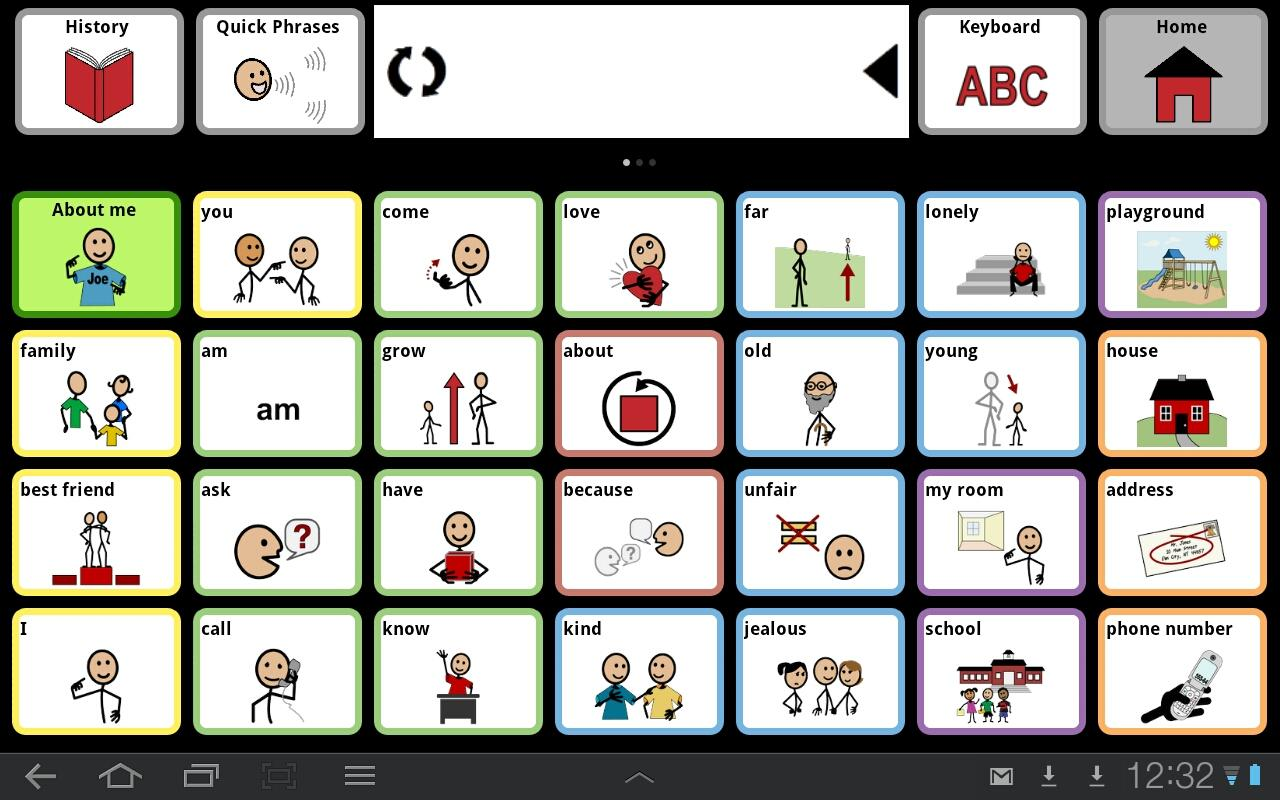
\includegraphics[width=150mm]{SonoFlex2}
\caption{Skjermdump av ASK programvaren Sono Flex}
\label{fig:SonoFlex}
\end{figure}


\section{Forskningspørsmål}
\label{sec:ResearchQuestion}

For å forske på mulige løsninger som forbedrer ASK-systemer vil en rekke funksjoner integreres i prototypen. Funksjoner som vil bli utprøvd og forsket på er følgende:


\begin{enumerate} 
\label{lst:features}
\item Forbedret visualisering. Undersøk mulige fordeler forskjellige visualisering effekter kan ha på navigering innen og mellom sider og kategorier.
\item Lydeffekter. Undersøk mulige fordeler forskjellige lydeffekter kan ha på navigering innen og mellom sider og kategorier.
\item Optimal organisering og kategorisering. Hvordan skal knapper bli organisert og kategorisert for best å legge til rette for og forenkle navigasjon
\item Brukertilpasning. Mennesker har forskjellige preferanser. Undersøk mulighetene for tilpasning av symbolstørrelse, animasjonsfart, farger o.s.v. 
\end{enumerate} 


Forskningen vil bli gjort ved å implementere et program basert på en eksisterende løsning. De ulike forbedringene beskrevet i (1),(2) og (3) vil bli integrert. Samtidig vil det også være mulighet tilpasse etter ønske (4). 


\section{Forskningsmetode}

Som nevnt i seksjon \ref{sec:ResearchQuestion}, er oppgaven å forbedre en type kommunikasjons programvare for mennesker med komplekse kommunikasjonsvansker. For å undersøke innvirkningene til de forskjellige funksjonene, vil de prøves ut på en testgruppe.
For å få til dette, vil et utvalg av deltakerene prøve systemet uten tilleggsfunksjonene, mens de gjenværende vil forsøke med funksjonene. Mens deltagerne kjører programmet vil deres interaksjon med bli automatisk lagret i logg. Informasjonen fra undersøkelsen vil vise hvordan brukeren navigerte og hvor lang tid de brukte. Dette kan igjen brukes til å verifisere om en funksjon er en forbedring eller ikke.



\chapter{Bakgrunn}

I dette kapittelet vil de viktigste konseptene, fenomenene og teknologiene bli beskrevet og eksisterende  forskning som er relevant for oppgaven. 

\section{Kommunikasjonsform: Symboler}

De som ikke har mulighet til å bruke skrift som kommunikasjonsform kan bruke tegnsystemer. Det eksisterer tre typer tegnsystemer: håndtegn(manuelle tegn) som innebærer å bruke håndbevegelser, materielle tegn vil si at en bruker fysiske objekter som brikker eller figurer og den siste er; grafiske tegn som innebærer at en bruker symboler. I denne rapporten er vil symboler bli brukt som kommunikasjonsform. Her representerer symboler et ord, frase, uttrykk eller setning. Ifølge ISAAC \cite{Tegnsystemer} er grafiske tegn brukt av mennesker med store bevegelsesvansker som gjør at de har utfordringer med å lage manuelle tegn, og mennesker med forståelsesvansker som følge av lærehemning.

De vanligste grafiske tegnsystemene på markedet er fotografi, pictogram, Picture Communication Symbols(PCS), Widgit, SymbolStix og Bliss \cite{GrafiskTegn}. I prosjektet brukes SymbolStix (se figur \ref{fig:katt}). Grunnen til dette er at Sono Flex bruker dette tegnsystemet.


\begin{figure}[ht!]
\centering
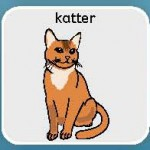
\includegraphics[width=50mm]{katt}
\caption{Et eksempel på et symbol som blir brukt i det grafisk tegnsystemet SymbolStix}
\label{fig:katt}
\end{figure}

\section{Interaksjonsform: Øyestyring}

Menneske-maskin-interaksjon fungerer ved at en person gir maskinen en kommando, og maskinen svarer med en respons. For at et menneske skal kunne gi en maskin ordre, er det nødvendig at maskinen har en inputenhet som tolker beskjedene fra brukeren, slik at at datamaskinen forstår dem.  Som regel er dette tradisjonelle enheter som tastatur og mus. Det eksisterer derimot mangfoldige måter å samhandle med en maskin på. I denne rapporten vil brukerinput bli gitt ved en øyestyringsenhet.  Ved å fange opp brukerens skuepunkt av et videokamera og infrarøde lys, er det mulig for maskinen å beregne hvor på monitoren personen ser. Dette gjør interaksjon mellom dem mulig. En knapp vil for eksempel bli aktivisert ved at brukeren ser på den en hvis periode. 




\section{Forskning}


\subsection{Organisering}


I 1926 kartla Smith\cite{Smith} barns vokabularutvikling fra alderen 1 til 5 år . Resultatene (se tabell \ref{fig:BarnVak}) viste at allerede i en alder av 3 er det vanlig å ha en gjennomsnittlig forståelse for cirka 900 ord. Forskningen er 88 år gammel, men viser omfanget av utfordringen barn har i møte med symbolbasert kommunikasjon. Mens et barn med taleevne kun trenger å finne ordet i hukommelsen, må barn som bruker symboler først finne det og deretter lokalisere det representative symbolet. 

I applikasjonen som skal utvikles vil symbolene bli presentert i en tabell. Antall symboler som får plass i tabellen begrenses av skjermens fysiske størrelse og at de må være store nok til at brukeren har mulighet til å se  og samhandle med dem. En slik tabell med symboler vil herfra bli referert til som en side. For hver setning brukeren vil uttrykke må han navigere seg igjennom flere av disse sidene for å finne symbolene som representerer ordene i setningen. Det er derfor essensielt at organiseringen legger til rette for akkurat dette, og ikke vanskeliggjør barnets evne til å lokalisere, velge og bruke symbolene.

\begin{table}[h]
\begin{tabular}{llllllllll}
\hline
Alder (År, Måneder) & 1 & 1,6 & 1,9 & 2,0 & 2,6 & 3,0 & 3,6  & 4,0  & 5,0  \\ 
Antall ord          & 3 & 22  & 118 & 272 & 446 & 896 & 1222 & 1540 & 2072 \\ 
Økning              & 2 & 19  & 96  & 154 & 174 & 450 & 326  & 330  & 532  \\ \hline
\end{tabular}
\caption{Tabell som viser vokabular vekst hos barn.  Smith \cite{Smith} sitert av Dale \cite{Dale} }
\label{fig:BarnVak}
\end{table}



Drager og Light \cite{aac} viser til at det inntil nylig var gjort lite forskning på layouts og organisering for barn eller om faktorene som spiller inn når det gjelder lokalisering og bruk av målobjektene. Målobjektet er symbolet som brukeren ønsker å uttrykke. Wilkinson og Jageroo \cite{Wilkinson2006} har undersøkt hvilke påvirkning farge har som en faktor når det kommer til organisering og hvordan elementer skal fordeles. De kom frem til at fargehint spiller en viktig rolle innen visuell prosessering  og hukommelse. Ved å legge til en farge ved elementene i tabellen over symboler, påvirket det nøyaktigheten og effektiviteten til barn i 4-5 års alderene i å finne målobjekt. Eksempelvis kan man gi symboler som representerer verb en grønn farge, adjektiv en blå, pronomen gul o.s.v. Fenomenet kalles Fitzergald Key og gjør at barn mer presist og raskere lokalisere målobjektet. Scally \cite{Scally} argumenterer for at farge ikke nødvendigvis er den eneste variabelen som må vurderes. Andre skjerm variabler som kan påvirke læring og bruk er: bakgrunn, kanter/grenser, form, tekstur, størrelse, posisjon, bevegelse og animasjon. Videre undersøkelser må til for å avgrense effektene av disse funksjonene for å kunne optimere designet til ask-systemer.


\subsection{Navigasjon}
\label{subsec:navigasjon}

Hvis en tar med alle typene frukt så vil det ikke være plass til alle symbolene på en side, dette gjør at de må deles opp over flere sider.Konsekvensen er at brukeren må ha mulighet til å navigere mellom disse sidene for å finne ønsket symbol. Siden antallet symboler det er plass til på hver side begrenses av skjermstørrelsen og brukerens syn, er spørsmålet hvor mange symboler bør plasseres på hver side med tanke på effektivitet. Drager og light med kollegaer undersøkte nettopp dette. Resultatene indikerte at barn i alderen 2-5 hadde større vanskeligheter for å lokalisere korrekt side fra en meny med 4 symboler enn en så lokalisere målobjektet når på korrekt side ut av et valg på 12 til 30 symboler, til tross for at sannsynligheten for å finne korrekt side er 25 prosent er mye større enn å finne korrekt symbol 0.03 - 0.08 når en først er på rett side.

For barn kan det å navigere være ekstra vanskelig. Dette kommer av flere grunner: (a) de må ha en konseptuell modell av de gjemte sidene i systemet i minnet. Med andre ord forstå hvordan de mest effektivt kan komme seg fra forsiden til ønsket symbol. (b) De må forstå forholdet mellom representasjon brukt på menysiden og de gjemte sidene i vokabularet. Er det symbolet som har bilde av et kjøkken eller av en butikk som leder til symbolet eple? I denne rapporten vil disse utfordringene bli undersøkt.




\chapter{Øyesporing}

Øyesporing refereres ofte til teknikken brukt til å fange og måle øyebevegelser \cite{Calibration}. Målet med dette kapittelet er å gi en beskrivelse av hvordan øyesporing fungerer og enheten som brukes i denne avhandlingen - samt en forklaring av viktige konsepter.


\section{Hvordan fungerer øyet?}

Å forklare hvordan øyet fungerer i detalj er utenfor denne rapportens omfang. Det vil derfor kun gis en høynivå forklaring av hvordan det fungerer for å kunne forstå det som er nødvendig i henhold til rapporten. 

\subsection{Synsfelt}

I en artikkel skrevet av Tobii \cite{Calibration} sammenlignes øyet med et fotoapparat på grunn av dens mange likhetstrekk. Når lys treffer et objekt reflekteres dette, det reflekterte lyset reiser så gjennom en linse og ender opp i øyet. Linsen prosjekterer lyset den mottar på en lyssensitiv overflate. Denne overflatens oppførsel er også det som skiller øyet fra fotoapparatet. For i motsetning til et kamera er ikke overflaten like sensitiv overalt i øyet.  Dette gjør at menneske kan tilpasse synet etter hvor mye lys som er tilgjengelig. En bieffekt er at det også resulterer i at menneske kun kan se klart i begrensede områder av synsfeltet. Figur \ref{fig:visueltArea} illustrerer hvordan synsfeltet hos menneske er delt inn etter klarhet. (F) representerer det foveale området. Dette er området man fokuserer på og oppfatter klarest. Det er hovedsaklig fra dette området visuell data hentes fra . (Pf) viser det parafovela omårdet, som kjennetegnes ved at uskarpheten øker til man kommer til det perifere området. (P) Det perifere området, også kjent som sidesynet, fungerer kun bra til å fange opp bevegelser og kontraster.

\begin{figure}[ht!]
\centering
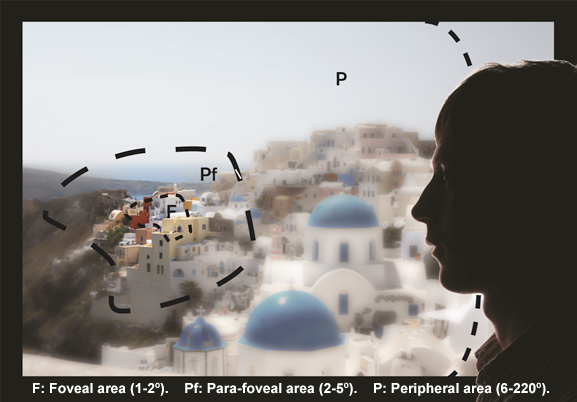
\includegraphics[width=65mm]{fovealArea}
\caption{Bilde/Illustrasjon av menneskelige synsfelt \cite{VisualImage}}
\label{fig:visueltArea}
\end{figure}

\subsection{Fikseringer og sakkader}

Det foveale området er som nevnt det området det registreres mest visuell data. Området står derimot for mindre 8 prosent av synsfeltet. Dette gjør at for å kunne innhente informasjon av interesse fra andre deler av synsfeltet må det flyttes inn i  det foveale området. For å gjøre det brukes øyeoperasjoner kalt fikseringer og sakkader. Fikseringer er pauser fra bevegelsen på et område, sakkader er hurtige bevegelser mellom fikseringene \cite{Calibration}.


\section{Hvordan fungerer øyesporing?}

Øyesporing er som tidligere nevnt teknikken brukt til å fange og måle øyebevegelser.
Det finnes derimot flere fremgangsmåter. I denne oppgaven vil det brukes en ikke-forstyrrende øyestyringsenhet. Dette gjør at brukeren i prinsippet ikke skal legge merke til enheten. For denne typen øyesporing er det mest vanlig å bruke en teknikk som heter Pupil Centre Cornea Reflection (\gls{PCCR}) \cite{Calibration}. Teknikken fungerer ved at en lyskilde belyser øyet for at refleksjonene skal bli klare og synlige. Et kamera tar deretter bilde av refleksjonene fra øyet. Bildet blir så brukt til å identifisere lysets refleksjon på hornhinnen og pupillen. Når en vet vinkelen mellom hornhinnen og pupillen er det mulig å regne ut en vektor. Vektoren sammen med andre geometriske egenskaper ved refleksjonene gjør det mulig å kalkulere ut blikkretningen(Der brukeren ser) \cite{Calibration}.


\subsection{Utfordringer}

En utfordring ved øyesporing er blunking. Blunking er et er en kortvarig sammentrekning av øyelokket, noe som gjør at øyet ikke vil gi refleksjon som kamera kan fange, og derfor ikke ha koordinater på hvor brukeren ser. Dette løses under analysen. Ved at og bruke koordinatene og øyets hurtighet før øyelokkene trakk seg sammen kan man ekstrapolere seg fram til en tilnærmet korrekt fiksering. 

\section{Tobii PCEye Go}

I denne rapporten brukes øyesporingsenheten Tobii PCEye GO, som vist i figur \ref{fig:tobiiPc}. Enheten kommer separat og kobles til datamaskinen via USB. Dette er som tidligere nevnt et ikke-forstyrrende apparat. Et eksempel på det motsatte ville vært et par briller som ble brukt til å spore øyebevegelser. 



\begin{figure}[ht!]
\centering
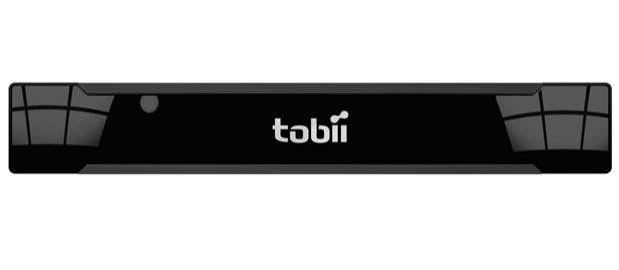
\includegraphics[width=50mm]{TobiiEyeGo}
\caption{Bilde av øyestyringsenheten Tobii PCEye Go}
\label{fig:tobiiPc}
\end{figure}


\subsection{Tobii blikkprogramvare}
\label{subsec:blikk}

Sammen med Tobii PCeye go følger det med programvare for å kontrollere applikasjoner som bruker sporingsenheten. Den består av følgende komponenter: 

\begin{itemize}
\item [Blikk interaksjonsserver] en sentral HUB som tilbyr klient applikasjoner øyesporingsdata. 
\item [Blikk interaksjons innstillinger] Et kontrollpanel for interaksjons innstillinger og oppgaver relatert til øyesporing
\item [Windows Kontroll] Tilbyr blikk interaksjon for standard Windows applikasjoner, ergo vanlige applikasjoner som ikke er laget for øyesporings interaksjon.
\end{itemize}

I denne rapporten vil kun førstnevnte være relevant. Ettersom applikasjonen er spesialisert til blikk interaksjon og ikke er en standard Windows applikasjon.

\subsection{Blikk Interaksjonsserver}

Blikk interaksjons-serveren er som nevnt i seksjon \ref{subsec:blikk} en HUB for programvaren, eller kjernen. Hovedformålet til denne komponenten er å samhandle med Øye-sporingsenheten og tilby interaksjonsfunksjonalitet for å kontrollere Windows baserte applikasjoner som vil bruke sporingsdata. I tilegg er det denne komponenten som tar seg av kalibrering, sporingsstatus - samt bruker og applikasjons innstillinger.

\subsection{Tobii Eye Control API }

Figur \ref{fig:overview} viser hvordan blikk interaksjonsserveren eksponerer funksjonalitet til en klient-applikasjon gjennom et APIet, som er kalt Tec API. For å ta i bruk TecAPIet tilbys to aksess punkter. Et gjennom .NET plattformen kalt TecClient og et for C dynamisk link library kalt MPACI.  Den praktiske betydningen, er at man kun kan bruke APIet ved å skrive i C eller .NET teknologier. I denne rapporten vil kun sistnevnte være interessant, altså .NET APIet kalt TecClient.


\begin{figure}[ht!]
\centering
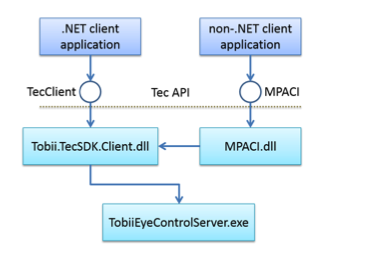
\includegraphics[width=100mm]{SoftwareArchitectureOverview}
\caption{Bilde som viser programvare arkitekturen til blikk programvaren}
\label{fig:overview}
\end{figure}


\subsection{TecClient}

TecClient støtter to GUI rammeverk; Windows Presentation Foundation (\gls{WPF}) og Windows Forms. 
 (kilde dokumentasjon).  Samhandling mellom applikasjonen og TecClienten skjer gjennom et konsept som de har valgt å kalle TecClients verktøykasse. De ulike verkøys klassene er presentert i figur \ref{fig:toolbox}. 

\begin{figure}[ht!]
\centering
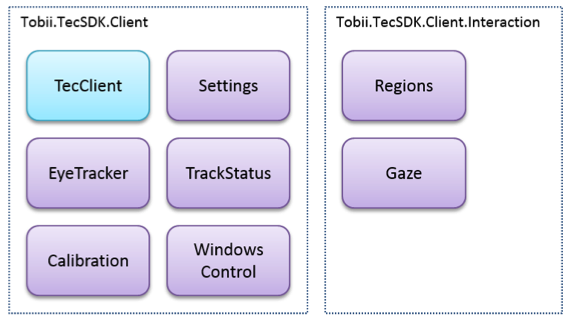
\includegraphics[width=100mm]{Toolbox}
\caption{Verktøy klassser som er tilgjengelige gjennom TecClient komponenten verktøyskasse}
\label{fig:toolbox}
\end{figure}


\subsubsection{EyeTracker}
Gir informasjon om den aktuelle øyesporingsenheten.

\subsubsection{Kalibrering}
Tilbyr tilgang til kalibrerings funksjonalitet og innstillinger som kan bli brukt for å kontroller hvordan kalibreringen er gjort.

\subsubsection{Settings}
Settings gir tilgang til bruker og klient innstillinger. Med mulighet til å hente nåværende bruker, alle bruker med funksjonalitet til å legge til og fjerne brukere og nåværende klient.

\subsubsection{Trackstatus}
Tilbyr metoder, egenskaper og hendelser for å kontrollere sporingsstatus vinduet. 


\subsubsection{Regions}
Tilbyr metoder, egenskaper og hendelser relatert til interaksjonsregioner. (1) Legge til og fjerne interaksjonsregioner, (2) hente informasjon om fokus og (3) søke etter interaksjonsregioner.

\subsubsection{Gaze}
Eksponerer blikkdata, både filtrert og ufiltrert. 



\chapter{Tobii Sono Flex}

I dette kapittelet vil den eksisterende løsningen sono flex bli diskutert. Det vil bli gitt en grundig analyse av problemstillingen og fremgangsmåte presentert.


\section{Tobii Sono Flex}
\label{chap:Tobii-Sono-Flex}


Programvaren som det tas utgangspunkt i heter Tobii Sono Flex,  og er et systematisert symbolforråd og et verktøy for alternativ og supplerende symbolspråk. Sono Flex har som mål å tilby et språk til personer som ikke enda kan lese og skrive. 

Applikasjonen fungerer som et tastatur, men istedenfor bokstaver er knappene ord med en visuell representasjon av ordet. Brukeren trykker på knappene som utgjør setningen han vil uttrykke, så vil programvaren gjøre om setningen til tydelig tale.  Systemet er spesielt utviklet for barn og unge med med sammensatte kommunikasjonsvansker, som trenger et ordforråd for å videreutvikle språk- og kommunikasjonsferdigheter. Sono flex kan ses på som en nybegynnerpakke med en lav læringskurve som skal gjøre brukeren klar for mer avanserte systemer. 


\subsection{Brukergrensesnitt}

Brukergrensesnittet til Sono Slex består av to hovedkomponenter: en menylinje og en symboltabell. 


\subsubsection{Menylinje}

Figur \ref{fig:menylinje} viser menylinjen.  Denne består av 5 elementer.  Kun de midterste er av interesse, disse  er statiske og følger applikasjonen hele tiden. Det hvite feltet i midten viser symbolene som brukerene har trykket på, og vil herved bli referert til som setningslisten. Symbolene som vises vil komme ut i form av tydelig tale ved å trykke på selve feltet. Knappen på venstre side av setningslisten (clear all), vil ved interaksjon tømme setningslisten. Mens knappen på høyre side vil kun fjerne det siste symbolet brukeren trykket på.


\begin{figure}[ht!]
\centering
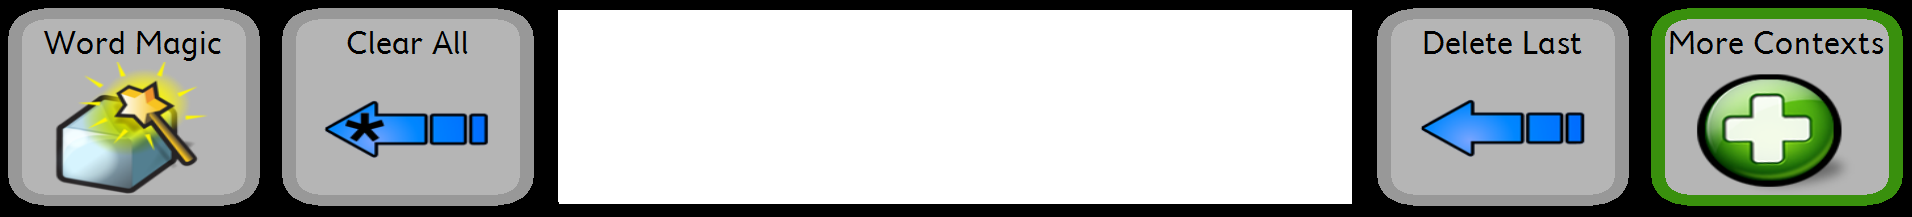
\includegraphics[width=100mm]{menylinje}
\caption{Skjermdump av menylinjen til programvaren Sono Flex}
\label{fig:menylinje}
\end{figure}




\subsubsection{symboltabell}
\label{subsubsec:symboltabell}

Figur \ref{fig:symbolgrid} viser applikasjonens symboltabell. Dette komponentet består av en tabell på 7 kolonner og 4 rader,  noe som gir 28 celler. I hver celle er det et Knapp bestående av et symbol og en tekstlig beskrivelse av symbolet. Ved å trykke på knappen vil en av tre ting skje avhengig av hvilken type knappen er av. Hvis knappen representerer et ord( "jeg",  "løpe",  "kake" o.s.v. ) så vil symbolet og medfølgende tekst vises i setningslisten i menylinje.  Hvis knappen har underliggende knapper som eksempelvis en ordklasse(verb,  substantiv)  eller kategori ("mat",  "frukt") så vil applikasjonen bytte ut de eksisterende symbolene i tabellen med ordene i ordklassen. Den siste typen symbol, er et navigasjonssymbol. Denne forekommer kun hvis det er for mange symboler i forhold til hvor mange det er plass til. Eksempelvis er det plass 28 symboler i tabellen, hvis da en kategori inneholder mer enn dette vil disse måtte fordeles over flere sider. Navigasjonssymbolet vil da være representert for å kunne bla mellom de ulike sidene.


\begin{figure}[ht!]
\centering
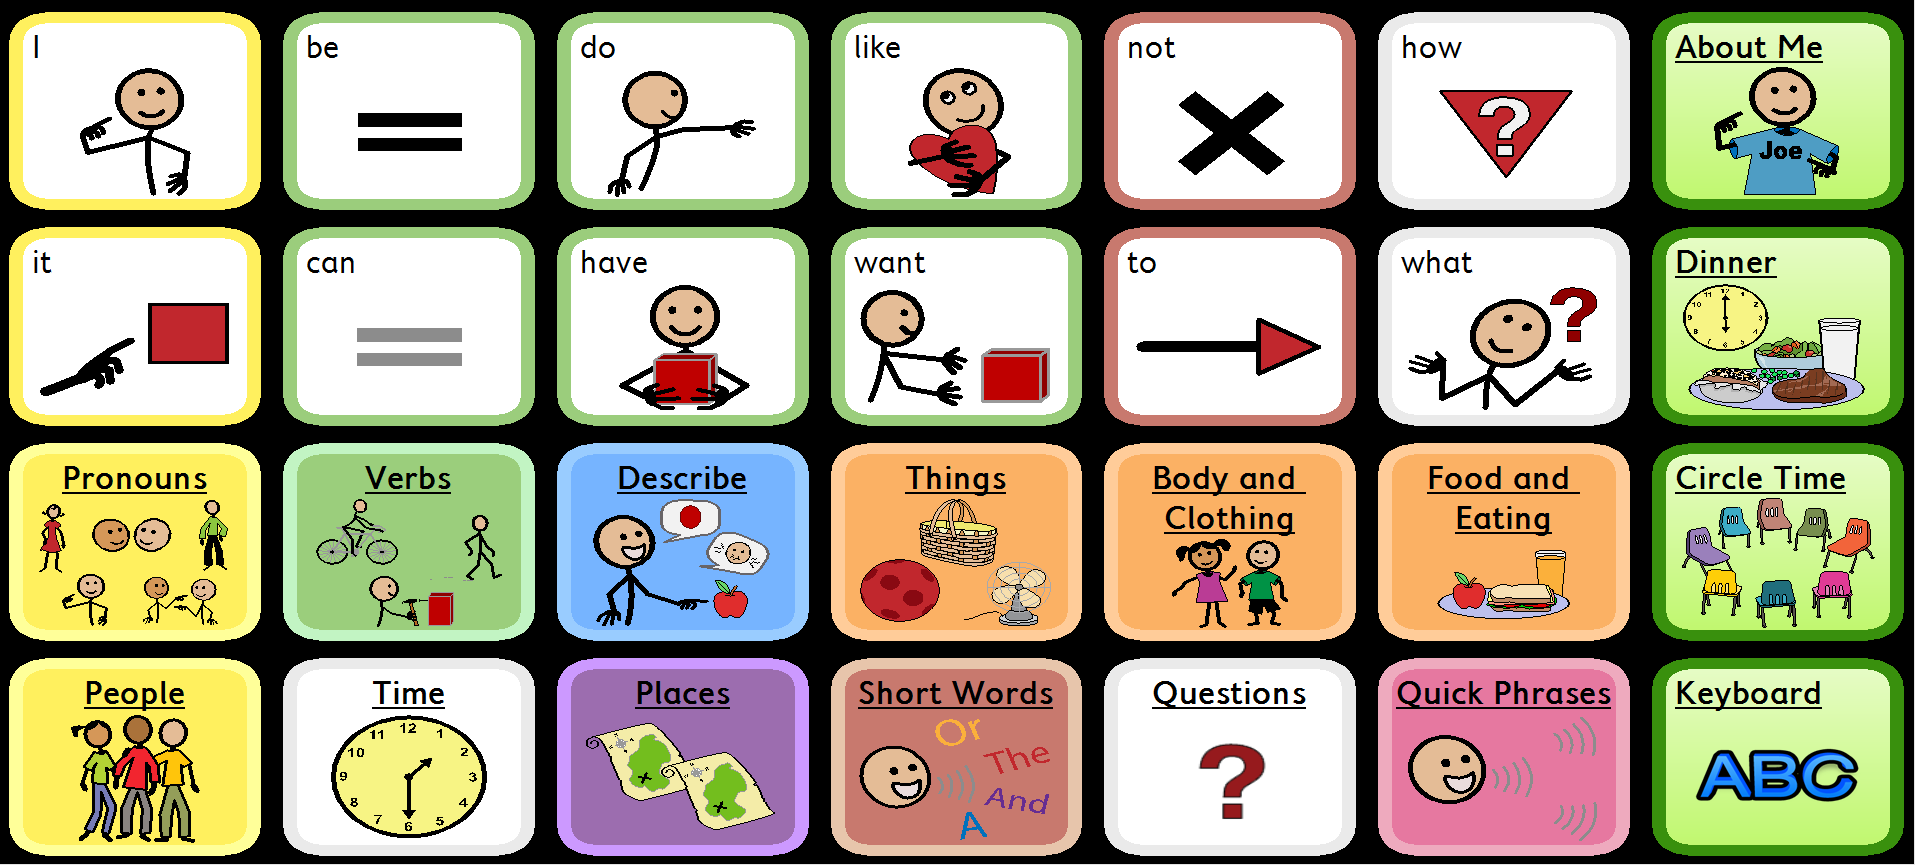
\includegraphics[width=100mm]{symbolgrid}
\caption{Skjermdump av symboltabellen til programvaren Sono Flex}
\label{fig:symbolgrid}
\end{figure}


\subsection{Brukerinteraksjon}

Sono Flex tilbyr to måter for brukerinteraksjon,  mus og øyestyring. Mus fungerer som vanlig ved at brukeren svever med musepekeren over ønsket knapp og venstreklikker for å aktivere. Ved øyestyring må brukeren fokusere blikket på ønsket knapp en gitt tid for at applikasjonen skal tolke det som et klikk. 

Det som skjer er at med engang brukeren fokuserer blikket på en knapp så starter en nedtelling. Figur \ref{fig:knapp-interaksjon} viser hvordan brukeren presenteres for hvor mye av nedtellingen som gjenstår.  Hvis brukeren ikke flytter blikket før nedtellingen har nådd null tolkes dette som et klikk.
For å gi brukeren beskjed om et godkjent klikk så dannes det en rød firkant rundt knappen. 

\begin{figure}[ht!]
\centering
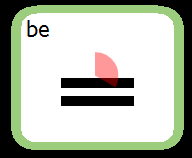
\includegraphics[width=50mm]{Knapp-interaksjon}
\caption{Skjermdump som viser hvordan nedtellingen på en knapp ser ut. Når den røde sirkelen er komplett oppfattes det som et klikk}
\label{fig:knapp-interaksjon}
\end{figure}


\section{Organisasjon og Navigasjon}

Som nevnt i seksjon \ref{subsec:navigasjon} så vil et barns vokabular være så stort at en nødvendigvis må fordele ordene over flere sider. Sono Flex har eksempelvis 106 ord under kategorien "Ting". Med tanke på at det maksimalt er plass til 28 ord på hver side så må disse fordeles og det må finnes en måte å navigere sidene. Løsningen har blitt en svært flat struktur med et hierarki på maksimalt 2 nivåer, ergo det finnes ikke underkategorier. Figur \ref{fig:hieraki-ting} viser hvordan dette fungerer i praksis. Når man trykker på kategorien "ting" så fylles tabellen med 27 ord som passer inn i kategorien "ting". Hvis man ikke finner ønsket ord på den første siden, navigerer man videre med knappen "neste side" og ordene i tabellen erstattes av nye ord. 


\begin{figure}[ht!]
\centering
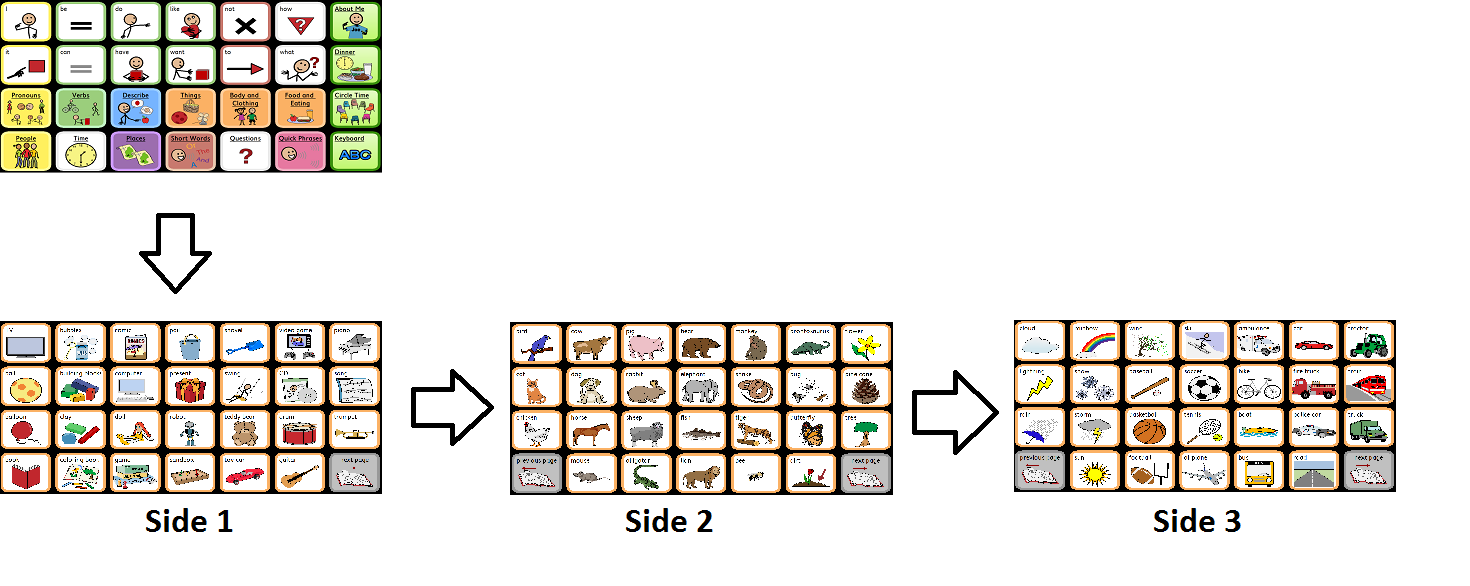
\includegraphics[width=140mm]{Symbgrid}
\caption{Skjermdump hierakiet til Sono Flex}
\label{fig:hieraki-ting}
\end{figure}

 
 
\chapter{Applikasjon} 
 
 
I dette kapittelet vil det bli gjort rede for utviklingen og de applikasjonen. 
 
 
\section{Utgangspunkt} 
\label{sec:utgangspunkt} 
 
 
Målet med forskningen er å undersøke potensielle forbedringer funksjonene beskrevet i seksjon \ref{sec:ResearchQuestion} kan ha på den eksisterende løsningen Tobii Sono Flex (\ref{chap:Tobii-Sono-Flex}). Det mest naturlige valget for å implementere disse funksjonene ville vært å ta utgangspunkt i den eksisterende kildekode og utvidet med nødvendig kode. Problemet var at plattformen som den eksisterende koden var bygget på hadde flere begrensninger og ville gjort det vanskelig å fått implementert mye av funksjonalitet som skulle undersøkes, spesielt gjelder dette animasjonene. Dette gjorde at utviklingen ble startet som et nytt prosjekt og at første del av utviklingen var å lage en forenklet prototype av den samme applikasjonen bare på en annet rammeverk. 
 
 
\section{Kravspesifikasjon} 
 
Prototypen som skal bygges skal ikke ha all funksjonaliteten som Sono Flex har, men nok til at den greier å utføre hovedoppgaven. Som vil si at brukeren har mulighet til å skrive setninger med symboler for så å gjøre om disse til naturlig tale. For å kunne gjennomføre dette er det flere mindre oppgaver som må implementeres.  De ulike kravene vil bli beskrevet etter prioritert der de første er de mest nødvendige og kjent som kjernefunksjonalitet, deretter vil funksjonalitet som hadde vært greit å ha, men som ikke er nødvendig for applikasjonen skal kjøre.  
 
 
\subsection{Funksjonelle krav} 
 
 
Øyesporing som interaksjon - Det skal være mulig å kun bruke øyene til å operere prototypen. Det vil si at en som kun har mulighet til å bruke øyesporing skal kunne ta i bruk alle funksjonene som en har ved å bruke datamus.  Effektivitet skal væreså lik som mulig mellom de to interaksjonsformene. 
 
 
Logging - I systemet skal det være mulig å kunne logge all interaksjonen en bruker gjør med programvaren. Denne funksjonen vil være nødvendig for å kunne gjennomføre testingen 
 
 
Brukertilpasning - Hver bruker skal ha mulighet til å kunne tilpasse programvaren etter sine preferanser.  
  
Tale - Systemet skal kunne gjøre om teksten til ethvert symbol om til tale fra høyttalerne. Dette vil bli aktivert på brukerens kommando. Dette vil typisk være når en bruker har fullført en setning. 
  
Internasjonalisering - Systemet skal minimum ha språkstøtte for engelsk, norsk, svensk, tysk og dansk. 
 
Animasjon - I prototypen skal det være animasjoner som blir aktivert når en bruker trykker på de ulike symbolene.  
Lydeffekter - Utenom talelyden, skal det også være lydeffekter som skal avspilles ved brukerinteraksjon.  
 
Symbol - Hver brikke skal bestå av et ord og et symbol som representerer dette på best mulig måte. 
 
 
\subsection{Ikke-funksjonelle krav} 
 
 
Responstid -  Programvaren er kompleks og det tar lang tid å skrive med symboler, det er derfor viktig at systemet responderer kjapt og ikke gjør slik at oppgaven tar lenger tid. Slik at når brukeren trykker på noe skal det føles som om programvaren svarer momentant. 
 
 
Brukervennlighet - Målgruppen består av barn med som har begrenset erfaring med å operere dataprogrammer. Det er derfor viktig at det legges vekt på det og programvaren utformes på en måte som er intuitiv for brukeren.   
 
 
Fleksibilitet - Kodebasen skal være tilrettelagt for vedlikehold og videreutvikling. Det er viktig at personer som ikke har deltatt i systemutvikling enklest mulig skal kunne forstå koden og på den måten enkelt kan legge til og fikse funksjoner. Programvaren skal også legge oppp til at det er enkelt og legge til animasjoner, lyd og nye brikker. 
 
Personvern - Brukerne av programvaren er en sårbar gruppe, det vil derfor være vikitg at sensitiv informasjon om disse ikke kommer på avveie. Det skal i utgangspunktet ikke lagres sensitiv data, men det hvis data lagres skal det lagres på en sikker måte. 
 
 
 
 
\section{Utvikling} 
 
 
I denne seksjonen vil teknologier og arbeidsområde bli beskrevet, som skal gi grunnlag for den neste seksjonen som vil gå mer innpå implementasjon valg og detaljer. 
 
 
\subsection{Rammeverk} //Skriv mer om  grunnen til at det eksisterende rammeverket ikke var nok 
 
 
Siden grunnen til at utviklingen begynte med blanke ark var begrensninger i det eksisterende rammeverket, var det viktig at den nye som applikasjonen skulle bygges på, ikke hadde dem. Valget ble derfor basert på at den var tilrettelagt for implementering av ønsket funksjonalitet. Det vil si god støtte for brukergrensesnitteknologi som animasjon, lyd og bildebruk. En begrensing var at rammeverket måtte være kompatibelt med øyestyringsenheten Tobii PCEye GO. Dette gjorde at alternativene ikke var mange.  
Valget falt derfor på Microsoft .NET. Grunnen til dette var at rammeverket oppfylte alle kravene og er godt dokumentert. 
 
 
Arkitekturen til .NET er omfattende og som en kan se utfra figur \ref{fig:net-arkitektur} er det flere programmeringsspråk og komponenter en kan velge å ta i bruk. Rapporten vil derimot kun gi informasjon om de ulike komponentene fra .NET som ble brukt og er nødvendig for videre lesning. 
 
 
\begin{figure}[ht] 
\centering 
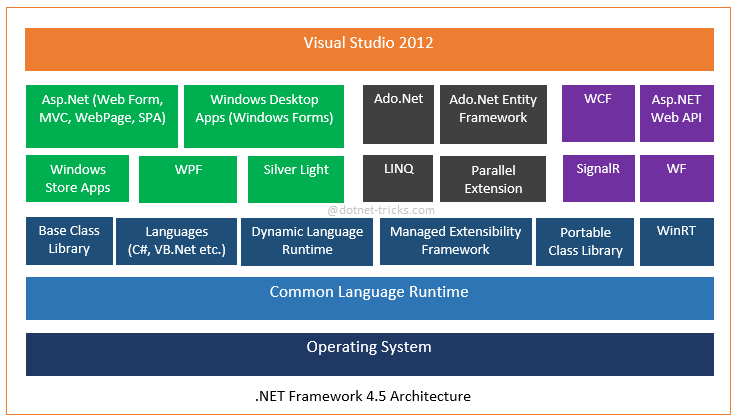
\includegraphics[width=140mm]{netframework45} 
\caption{Diagram som viser arkitekturen til .net rammeverket versjon 4.5} 
\label{fig:net-arkitektur} 
\end{figure} 
 
 
\subsection{Teknologi} 
 
 
Innenfor .NET sto valget mellom teknologiene Windows Store Apps, Windows Presentation Foundation(\gls{WPF}), Windows Forms og Silverlight.  Windows Forms ble utelukket ettersom dette er teknologien som Sono Flex er bygget på og som hadde begrensinger som gjorde at flere ønskede funksjoner ble vanskelig å implementere. Windows Store Apps hadde mye av den ønskede funksjonaliteten, samtidig som den fortsatt vedlikeholdes. For å distribuere slike applikasjoner brukes Windows Store. Problemet er at for å få publisert applikasjonen der, kreves godkjenning av Windows. En tidkrevende prosess, og med tanke på at applikasjonen antageligvis vil oppdateres hyppig kan dette bli et problem. Dette i sammenheng med at disse applikasjonene ikke er kompatible med Windows 7\cite{Windo0:online} gjorde at denne teknologien ble valgt bort. Til slutt sto valget mellom Silverlight og WPF. Silverlight er en kryssplattform, kryss web implementasjon av .NET rammeverket som har god støtte for grafiske elementer, animasjon og audio, og derfor en god kandidat. Funksjonaliteten i silverlight er et subset av WPF, som vil si at WPF minst har samme funksjonalitet som silverlight. Med unntak av Deep Zoom en funksjon som applikasjonen ikke hadde spesifikk behov for \cite{WPFvsSilverlight:online}. I tillegg til å tilby mer funksjonalitet var også bruk av wpf sammen med øyesporingsenheten beskrevet i enhetens dokumentasjon. Noe som vil gjøre prosessen med å integrere øyesporing i applikasjonen lettere. Dette gjorde at vi bestemte oss å utvikle i WFP. 
 
 
 
 
\section{Windows Presentation Foundation} 
 
 
Ifølge Adam Nathan \cite[p.~9]{WPFbook}, programvare arkitekt hos Microsoft er grunnen til at WPF ble lansert er at til tross for grafikk maskinvare hele tiden har blitt bedre og billigere og  forbrukerens forventninger fortsatt å stige, så er det ingen som har adressert vanskeligheten med å lage moderne brukergrensesnitt ref{Adam nathan bok side 9}.  Han argumenterer med at ja det fantes utviklere på tiden som for eksempel brukte bitmap bilder til å lage kulere knapper istedenfor å bruke standardknapp kontrollen. Problemet er at disse formene fort tilpasning ikke bare kan være ressurskrevende å utvikle, men også gi en dårligere brukeropplevelse. Nathan forteller derfor at Microsoft innså at det var et behov for noe helt nytt som ikke hadde de samme begrensningene som GDI+ og USER ga, men som samtidig hadde produktiviteten som folk likte fra rammeverk som Windows Forms. Sammen med at applikasjoner bygget med HTML og Javascript steg i popularitet. Trengte Windows en teknologi som var like morsom og enkel å bruke som disse, men samtidig som den utnyttet kraften den aldri-stoppende utviklingen av maskinvare har gitt. Resultatet ble Windows Presentation Foundation. 
 
 
   
\section{Arbeids område} 
 
 
For å automatisere mye av utviklingen ble det valgt å bruke utviklingsmiljøet Visual Studio 2013 \cite{2013-1:online}. Grunnen til at Visual Studio ble valgt er det for at i tillegg til å ha koderedigeringsverktøy og debugger, så har den også en WPF designer\cite{What8:online}. Denne designeren tilbyr flere hjelpemidler for å effektivisere prosessen med å lage brukergrensesnitt. Blant annet kan man velge mellom å kode de forskjellige elementene eller man kan dra dem inn fra et sidepanel. Den viktigste er derimot design vinduet, som til enhver tid viser hvordan brukergrensesnitt blir uten å måtte kjøre koden\cite{WPF D1:online}. 
 
 
For versjonskontroll ble det på grunn av erfaringsmessige årsaker brukt git\cite{AboutGit:online}. Til å ta backup av git filene ble den web-baserte tjenesten Bitbucket brukt. Grunnen til dette var mye av koden fra Tobii Dynavox var konfidensiell og Bitbucket tilbyr gratis hemmelig oppbevaring. 
 
 
\section{eXtensible Application Markup Language} 
 
 
 WPF bruker eXtensible Application Markup Language (\gls{XAML}), som er et XML-basert språk til å definere og kombinere ulike grensesnittelementer. Figur \ref{lst:myLabel} viser hvordan et vindu med en knapp er definert i XAML. Resultatet kan ses i figur \ref{fig:xamlButton}.  
 
 
\begin{lstlisting}[language=java,caption={Kodesnutt skrevet i XAML som viser en enkel applikasjon med en knapp} 
\label{lst:myLabel}, belowcaptionskip=4pt] 
<Window xmlns="http://schemas.microsoft.com/winfx/2006/xaml/presentation" Title="Window with Button"  Width="250" Height="100"> 
 
 
  <Button Name="button" Click="button_Click">Click Me!</Button> 
   
</Window> 
\end{lstlisting} 
 
 
\begin{figure}[ht!] 
\centering 
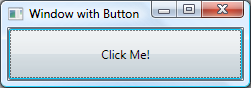
\includegraphics[width=100mm]{xamlButton} 
\caption{Skjermdump av det applikasjonen som blir gjengitt ved kjøring av kodefnutt \ref{lst:myLabel}} 
\label{fig:xamlButton} 
\end{figure} 
 
 
 
 
For å kunne samhandle med de grafiske objektene definert i XAML filen opprettes det alltid en tilhørende kodefil sammen med denne. Kodefilens formål er å ta seg av data og logikk for å ha et klart skille mellom utseende-spesifikk kode og oppførsel-spesifikk kode. For eksempel så vil en knapp sitt utseende og plassering bli definert XAML filen, mens hvordan data blir påvirket av interaksjon med knappen blir definert i den tilhørende kodefilen. 
 
 
Den tilhørende kode-filen til XAML koden beskrevet i kodesnutt \ref{lst:myLabel} er vist i kodesnutt \ref{lst:backbutton}. Ved å trykke på knappen bildet vil metoden button\textunderscore Click i kodefilen bli kalt og en dialogboks vist til brukeren. 
 
 
En XAML fil definerer som tidligere nevnt grafiske objekter som vindu, side eller brukerkontroll, men for at en bruker skal kunne samhandle med applikasjonen trengs de 
 
 
Vindu inneholder er en konteiner som inneholder alle applikasjonens grafiske elementer. En 
 
 
For å håndtere logikken og interaksjon med brukergrensesnittet,  definert i XAML, brukes det en kode fil. For hver XAML   Dette gjør at koden har et klart skille mellom utseende-spesifikk kode og oppførsel-spesifikk kode. 
 
 
Som tidligere nevnt defineres brukergrensesnittet i XAML, 
 
 
WPF oppfordrer til å skille mellom utseende spesifikk kode og oppførsel-spesifikk kode ved at grafiske elementer skrives i XAML og interaksjonen  kun brukes til generere  
XAML brukes til å generere brukergrensesnitt,  
Hver XAML-fil har en tilhørende kode-fil for håndtering av hendelser og oppførsel. Dette gjør at koden har et klart skille mellom utseende-spesifikk kode og oppførsel-spesifikk kode. Den tilhørende kode-filen til XAML koden beskrevet i kodesnutt \ref{lst:myLabel} er vist i kodesnutt \ref{lst:backbutton}. Ved å trykke på knappen bildet vil metoden button\textunderscore Click i kodefilen bli kalt og en dialogboks vist til brukeren. 
 
 
\begin{lstlisting}[language=java,caption={falafel} 
\label{lst:backbutton}] 
 void button_Click(object sender, RoutedEventArgs e) 
        { 
         Viser en dialogboks naar knappen trykkes 
        MessageBox.Show("Hallo!"); 
        } 
\end{lstlisting} 
 
 
 
 
\section{Model View ViewModel} 
 
 
En viktig del av oppgaven var å bygge en prototype som Tobii Dynavox kunne bygge og teste videre på. Det var derfor en forutsetning at kildekoden var tilrettelagt for vedlikehold og videreutvikling. For å gjennomføre dette valgte vi å følge arkitekt mønsteret Model view viewmodel (MVVM). Grunnen til at vi valgte nettopp dette foran andre mønster, som for eksempel Model View Contoller(MVC)\{MVC a2:online} eller Model-View-Presenter(MVP)/cite{The M4:online} er fordi WPF er designet for å lage applikasjoner med MVVM, Microsoft brukte selv MVVM til å utvikle WPF \cite{THEM6:online}. Det er mulig å bruke andre mønster, men det virket med dette argumentet mest logisk og velge MVVM. 
 
 
MVVM skal hjelpe utviklerne til med å separere forretnings- og presentasjonslogikk i applikasjonen fra brukergrensesnittet \cite{Im1online}. Ved å vedlikeholde er klar skille mellom applikasjons logikk og brukergrensesnitt skal det ifølge Microsoft \cite{Im1online}, gjøre det enklere å teste, vedlikeholde og videreutvikle.  
 
 
\begin{figure}[ht!] 
\centering 
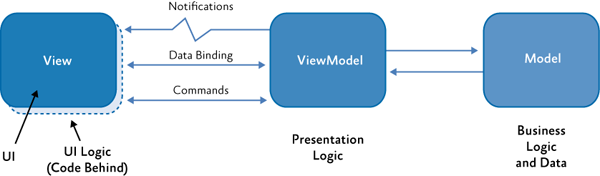
\includegraphics[width=100mm]{Mvvm} 
\caption{Illustrasjon som viser tre MVVM klasser og hvordan interaksjonen mellom dem\cite{Im1online}} 
\label{fig:mvvm} 
\end{figure} 
 
 
Figur \ref{fig:mvvm} viser de tre MVVM klassene view, view-model og model, og interaksjonen mellom disse. I view klassen defineres de visuelle elementene som vinduer, knapper, tekst, farger og organiseringen av dem. Med andre ord, selve brukergrensesnittet.  For at en bruker skal kunne utføre kommandoer og hente data gjennom et view, brukes det i WPF, databindings uttrykk som blir evaluert opp mot viewets gitte datakontekst. I MVVM vil datakonteksten være satt til viewmodellen. Det vil si som figur \ref{fig:mvvm} viser, at alle former for kommandoer, notfikasjoner og databinding skjer gjennom viewmodellen. Et view vil typisk kun forholde seg til en viewmodel, altså et en-til-en relasjon\cite{ite{THEM6:online}.   
 
 
Mens viewet bestemmer hvordan applikasjonen skal se ut, så bestemmer viewmodellen hvordan funksjonaliteten skal være \cite{THEM6:online}. Det er i viewmodellen at egenskaper og kommandoer som viewet kan binde seg opp mot er implementert. Når data  da endres vil view bli varslet og oppdatert deretter(Notified i figur \ref{fig:mvvm}) . På samme måte vil viewet kalle på viewmodellen om at en kommando må kjøres hvis for eksempel en bruker trykker på en knapp. Det er også Viewmodellen sitt ansvar og koordinere interaksjoner med viewet med de modellene som trengs. Det vil si at viewmodellen kan eksponere modellen direkte til viewets slik at de kan bindingen kan skje direkte til dem. Samtidig kan viewmodellen også manipulere data fra modellen , som for eksempel å kombinere to verdier. Eksempel kan være å sette sammen fornavn og etternavn fra en Person modell. Mens forholdet mellom View og Viewmodellen typisk er en-til-en, så vil ViewModellen ha en en-til-mange relasjon.  
 
 
\subsection{MVVM light} 
 
 
//Siden ny utvikling og lage en testplattform, viktig at kode var optimalisert 
//Mvvm passet best skille mellom logikk og blablabla 
//Vikitg å få med design time data, side applikasjonen er svært design tung 
//Finn fordeler 
//mvvm light  - IOC container, design data. 
//Arkitektur 
 
 
 
 
 
 
\section{Utvikling}  
 
 
I seksjon \ref{sec:utgangspunk} ble teknologien som ble brukt til å utvikle prototypen diskutert. I denne seksjonen vil arkitektturen og de viktigste utviklingsdetaljene  bli drøftet.  
 
 
\subsection{Arkitektur} 
 
 
Figur \ref{fig:arkitektur} viser et forenklet bilde over hvordan klassene i kodebasen er koblet sammen. Med forenklet så menes det at flere hjelpeklasser og tredjeparts bilioteker er med i diagrammet. I tilegg så har ikke Views blitt tatt med i diagrammet, men for hver ViewModel så er det View som representerer det.  
 
 

 
\begin{figure}[ht] 
\centering 
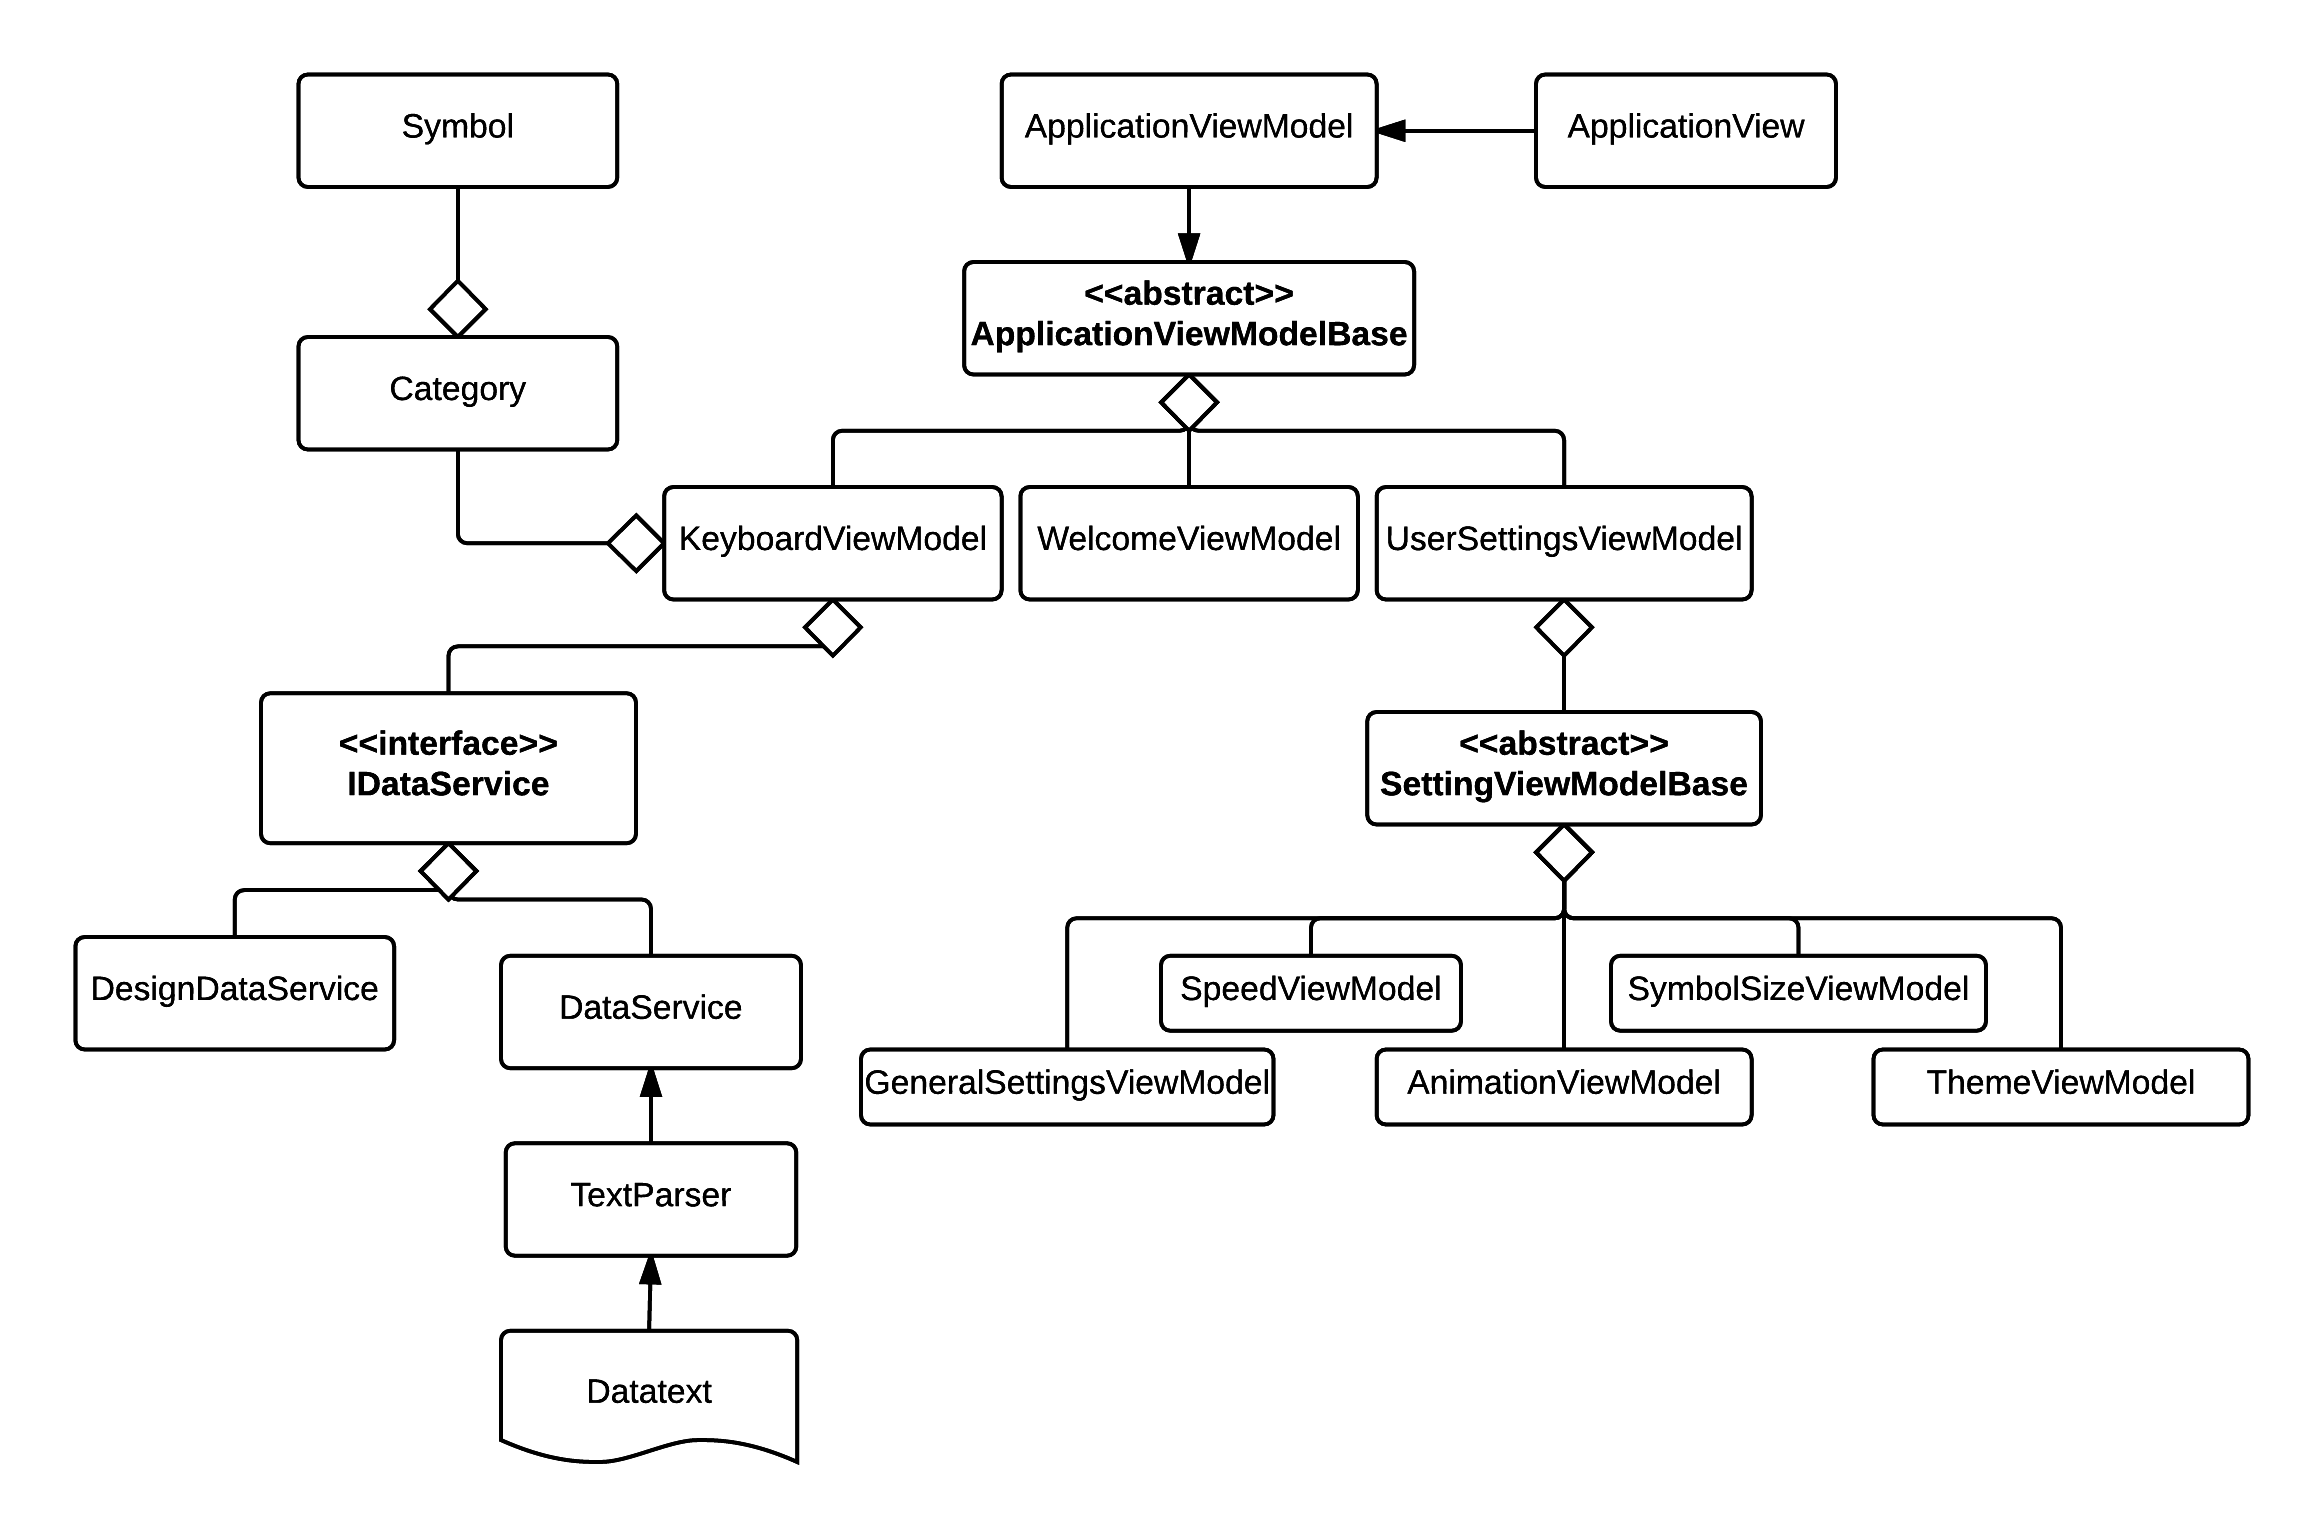
\includegraphics[width=140mm]{Arkitektur} 
\caption{Figur som viser et overordnet bilde av hvordan de ulike klassene henger sammen} 
\label{fig:arkitektur} 
\end{figure} 
 

 
ApplicationViewModel er vinduet som åpnes når programmet startes. Denne klassen fungerer som en kontainer for applikasjonen og bestemmer kun applikasjonsvinduets størrelse og navigasjon mellom de andre viewmodellene Keyboard, Welcome og UserSettings.  
 
 

\begin{listing}[ht] 
\inputminted[fontsize=\footnotesize, frame=lines,framesep=2mm,baselinestretch=1.2,bgcolor=lightgray,linenos]{xml}{Code/ApplicationContainer.xml} 
\caption{Utdrag fra kode som viser hvordan kontainer er satt opp} 
\label{listing:Kontainer} 
\end{listing} 
 
 
\begin{listing}[ht] 
\inputminted[fontsize=\footnotesize, frame=lines,framesep=2mm,baselinestretch=1.2,bgcolor=lightgray,linenos]{csharp}{Code/CurrentApplicationView.cs} 
\caption{Utdrag fra kode som viser hvordan kontainer er satt opp} 
\label{listing:CurrentAppView} 
\end{listing} 
 
 
 
 
Figur \ref{listing:Kontainer} viser hvordan ContentControl elementet i ApplicationView fungerer som en kontainer ved at innholdet er bundet til egenskapen CurrentViewModelBase. Som vil si at innholdet i ContentControl vil basere seg på hva som er satt som CurrentViewModelBase i ApplicationViewModel. Figur\ref{listing:CurrentAppView} viser hvordan denne egenskapen er implementert i Viewmodellen. Utfra koden så kan man se at til forskjell fra viewet, som hadde en referanse til egenskapen, så er det ingen direkte referanse fra viewmodellen til viewet. Dette er for å følge prinsippet til MVVM om at viewmodellen ikke skal ha noe kjennskap til Viewet, som gjør koden løs koblet(les: loose coupled). Men siden dette er en verdi som antakeligvis vil endre seg i løpet av kjøretiden er det nødvendig at Viewet blir gjort oppmerksom på forandring. Dette skjer ved å avfyre RaisePropertyChanged, dette kallet vil varsle rammeverket om at en endring har skjedd. Når da Viewet har en binding til denne egenskapen vil han bli oppmerksom på endringen og oppdatere deretter \cite{MVVM4:online}. 
 
CurrentViewModelBase er av typen ApplicationViewModelBase som vil si at det som er i kontaineren må være av nettopp denne typen. ApplicationViewModelBase er som man ser utifra figur  en abstrakt og har kun en abstrakt metode for å hente navn.  Det vil si at de klassene som arver fra ApplicationViewModel må implementere metoden. Fra figur kan man se at de klassene som arver fra ApplicationViewModel og med det har mulighet til å være i kontaineren er, KeyboardViewModel, UserSettingsViewModel og WelcomeViewModel. Sammen representerer disse hoved funksjonaliteten til programvaren. KeyboardViewModel er hoveddelen av applikasjonen, det her en bruker har mulighet til å skrive setninger med å trykke på de ulike symbolene for så å gjøre dem om til tale. I UserSettings kan en bruker se og endre på de ulike innstillingene. Mens \texttt{WelcomeViewModel} er kun laget for testingen og funksjonaliteten er begrenset til at en bruker kan velge alder og kalibrere øyesporingsenheten. 
 
 
 \subsection{Skrivebordet}
 
KeyboardViewModel og KeyboardView utgjør sammen det som blir kalt skrivebordet. Skrivebordet er den delen av programvaren som tilbyr hovedfunksjonaliteten, å la en bruker kunne skrive setninger. For å gjøre dette så må er det en del viktig elementer som må være tilstede. Man kan si at skrivebordet skal være en digital representasjon av det klassiske tastaturet. Der det er ord med symboler istedenfor bokstaver, og trykk skjer ikke ved fysisk trykk, men ved å se på knappen over en periode. Utenom dette skal funksjonaliteten være mye den samme. De mest nødvendige funksjonene som å kunne viske og bygge setninger må ihvertfall være tilstede. I tillegg må prototypen ha mulighet for å kunne presentere setningene som lyd. 

\begin{figure}[ht!] 
\centering 
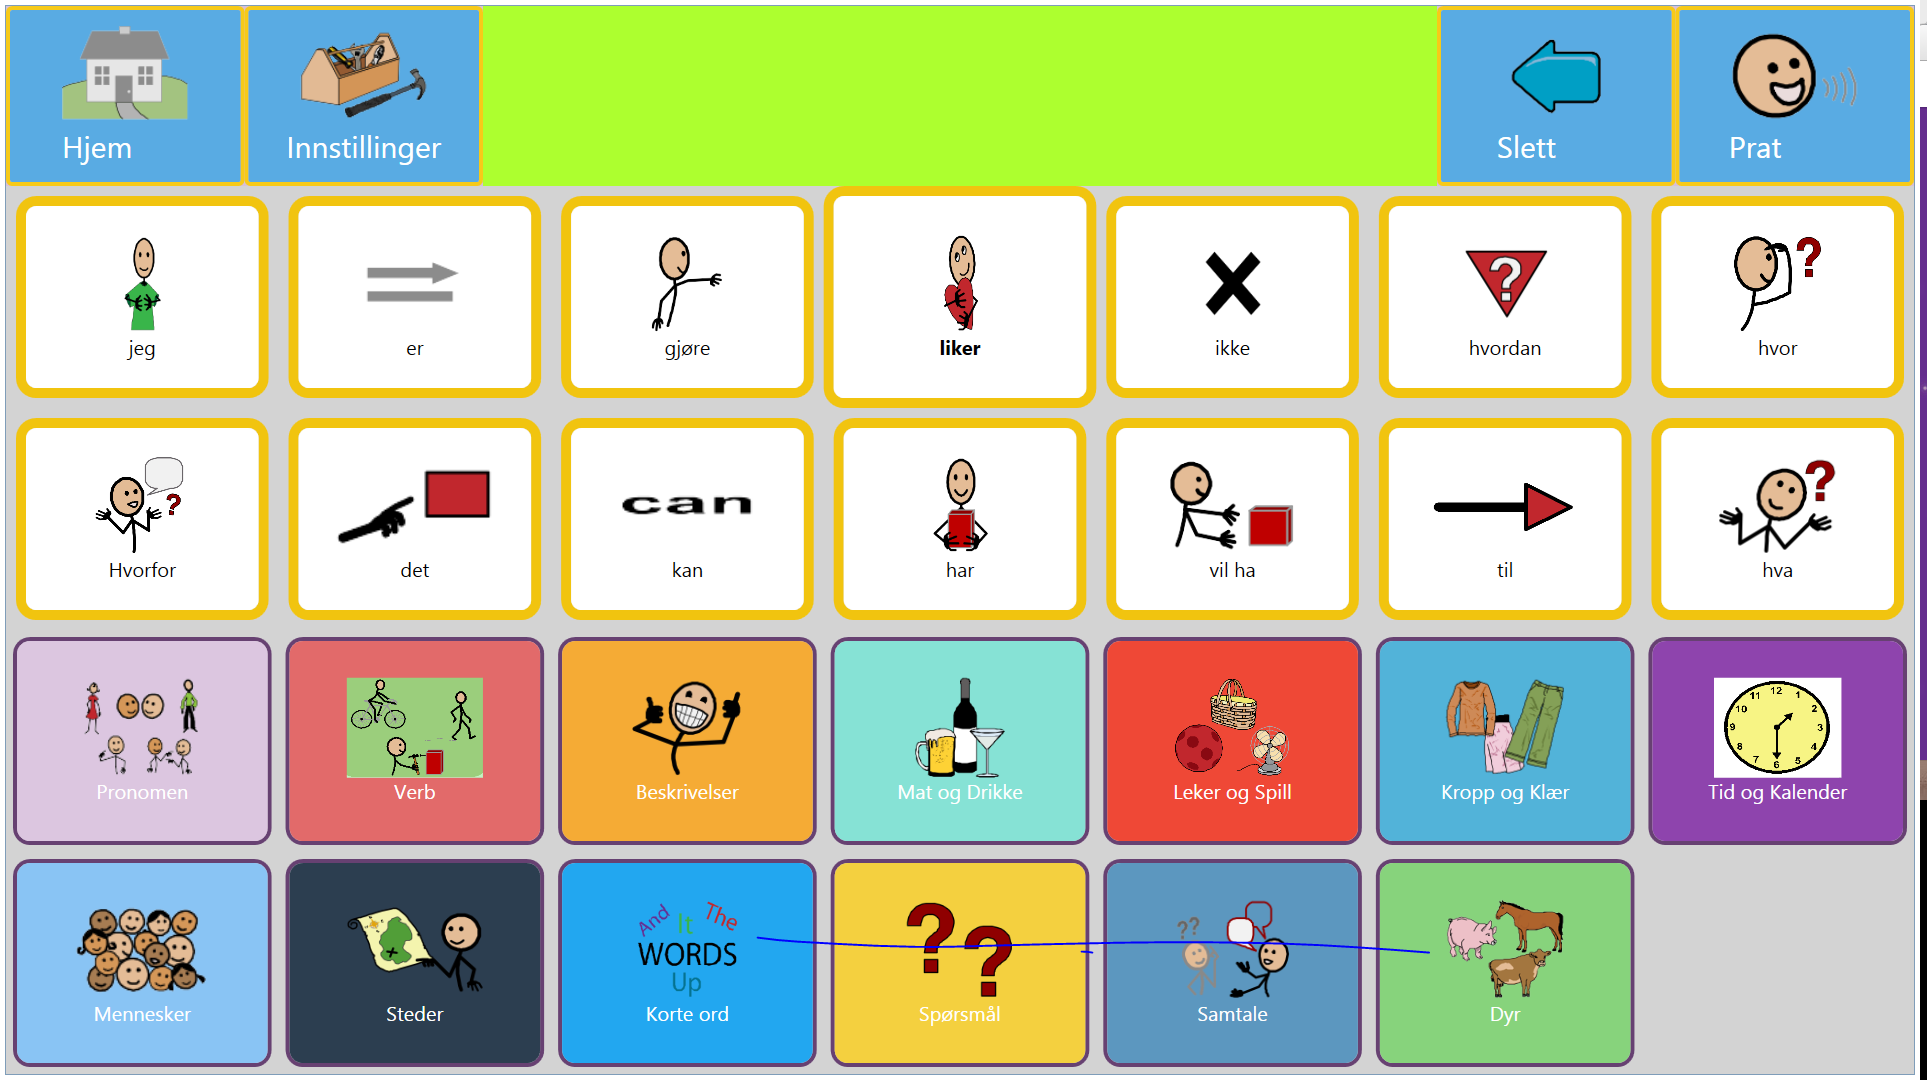
\includegraphics[width=100mm]{skrivebord} 
\caption{Skjermdump av skrivebordet i prototypen} 
\label{fig:skrivebord} 
\end{figure} 
 

\subsubsection{Innlesning}


For å kunne skrive med skrivebordet er det nødvendig at det er fullt opp med ord og symboler. For å gjøre dette blir metoden texttt{GetInitialPages} vist i figur .. kalt fra konstruktøren. Denne metoden kaller så igjen på metoden GetCategory("Frontpage") i klassen \texttt{Dataservice} vist i figur ... Grunnen til at ViewModellen ikke kun direkte henter symbolene er fordi de er lagret på et tekstdokument. Så for å separere data fra presentasjon- og forretningslogikk så brukes det et data tilgang lag i mellom. For å gjøre om tekstfilen til strukturerte data bruke datatjenesten klassen TextParser til å tolke den. 


\subsubsection{Data og innlesning av dem}

Programvaren skal strebe etter å kunne tilby brukeren ordene han har lyst å bruke. Noe som kan være utfordrende med tanke på at et barns vokabular allerede i alder av 5 år kan være opp i mot XXXX ord. Med tanke på hvilke ord som er i vokabularet vil variere  fra person til person så må programvaren ha en god del mer enn dette. I tillegg til  må også programvaren tilby et bilde for vært av ordene. 

En naiv fremgangsmåte for å lage brikkene er å statisk initialisere hver brikke med et ord og bilde. Problemet med dette er først og fremst at XAML koden blir unektelig lang som følge av at en må skrive en knapp for vært tilfelle. Den at en også må inn i koden for å gjøre endringer eller legge til nye ord, er ugunstig ettersom det er en ressurskrevende prosess. Løsningen på dette var å oppbevare alle ordene i en separat fil for å skille mellom brukergrensesnitt og data. For at maskinen skulle ha mulighet til å lese dataene ble de lagret i JavaScript Object Notation(JSON) format. JSON er ifølge sine egne nettsider \cite{JSON7:online} et lettvekt data-utvekslings format. Som er lett for mennesker å lese og skrive og det er lett form maskiner å tolke og generere. Kode \ref{listing:jsonfile} viser et utdrag fra json filen hvor ordene og stien til bildet som representerer ordet, er lagret. Filen består i en liste med JSON objekter som har attributtene Name og Image. Der Name er ordet og image er stien til symbolet. Dette er bare et lite utdrag fra filen og viser kun det som ville tilsvart fire brikker i programvaren. Det første objektet "I" er et ord, mens de tre neste er kategorier. Hver kategori består av flere ord. Ordene som tilhører en kategori er lagret i en egen fil i en mappe med samme navn. Figur \ref{jsonstructure} viser strukturen på filene, der hver kategori har sin egen mappe. Dette gjør at data hentes "just-in-time". Det vil si at istedenfor at ordene ligger i minnet til enhver tid, så hentes de kun når ved behov. Eksempelvis hvis en bruker trykker på kategorien "Food and Drink" så vil ordene hentes fra "FoodAndDrink.json" i mappen "FoodAndDrink". Noe som sparer på minnet, men som kan forringe kjøretiden. For når det er snakk om så store mengder data som alle ordene ville gitt, er det ikke gunstig å bevare dem i minnet. 


\begin{listing}[ht] 
\inputminted[fontsize=\footnotesize, frame=lines,framesep=2mm,baselinestretch=1.2,bgcolor=lightgray,linenos]{json}{Code/JSONfile.json} 
\caption{Utdrag fra filen som inneholder ord og sti til bilde som representerer det i JSON format} 
\label{listing:jsonfile} 
\end{listing} 
 
 
 \begin{figure}[ht!] 
\centering 
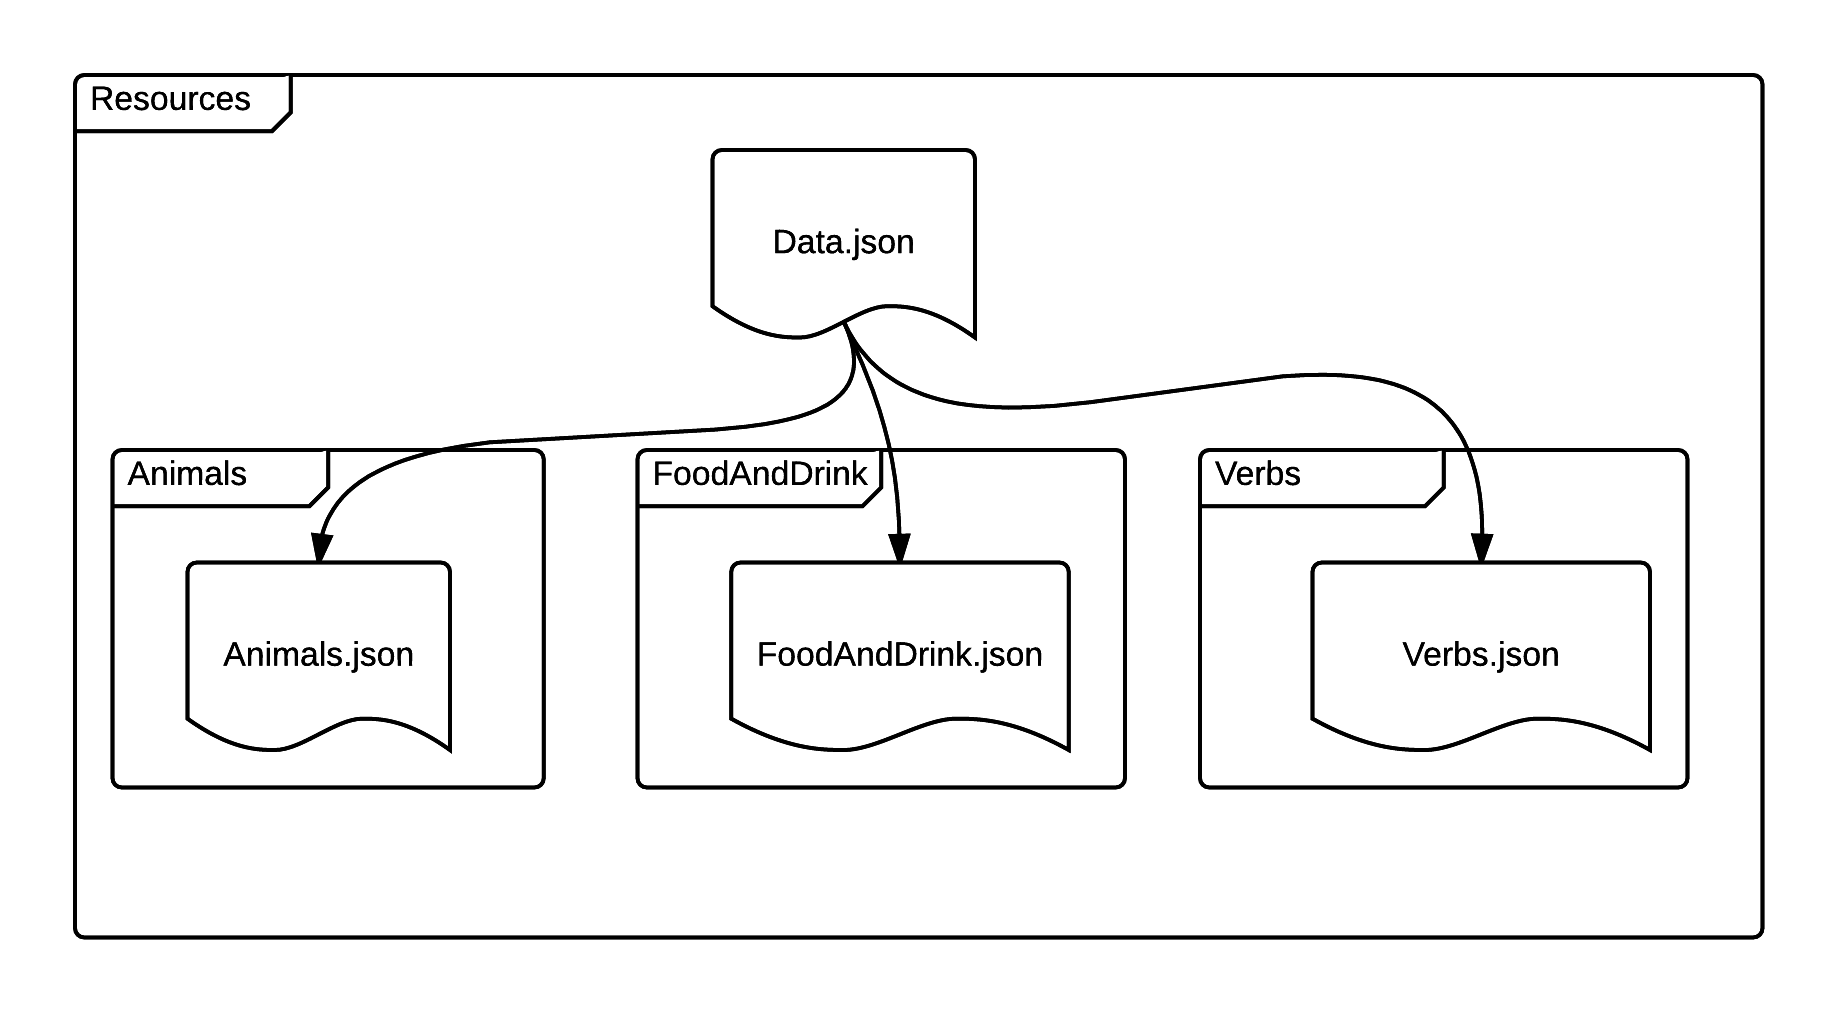
\includegraphics[width=100mm]{JsonStructure} 
\caption{Bilde av dokumentet hvor de ulike symbolene er registrert} 
\label{fig:jsonstructure} 
\end{figure} 


For å kunne ta i bruk objektene definert i tekstfilen må de tolkes fra JSON format til .NET objekter. Denne prosessen, å trekke ut datastrukturer fra bytes, kalles deserialisering. For å gjøre dette har vi brukt et tredjeparts rammevekt kalt JSON.net \cite{Json.0:online}. Det finnes en innebygd funksjon i .NET kalt DataContractJsonSerializer \cite{DataC3:online} som også greier å deserialisere et JSON dokument. Grunnen til at JSON.NET ble brukt er fordi i dette biblioteket er det mulighet for å automatisk deserialisere en helt liste av JSON objekter til .NET liste uten å manuelt måtte legge inn objektene. Ifølge utviklerens egne nettsider skal rammeverket være 50 prosent kjappere enn DataContractJsonSerializer, men ytelsen er avhengig av hvilke datasett som brukes, og har ikke vært en faktor i avgjørelsen. 


\begin{listing}[ht] 
\inputminted[fontsize=\footnotesize, frame=lines,framesep=2mm,baselinestretch=1.2,bgcolor=lightgray,linenos]{csharp}{Code/JSONparser.cs} 
\caption{Koden som konverterer JSON filen til en IList} 
\label{listing:JsonParser} 
\end{listing} 


Koden i figur \ref{listing:JsonParser} deserialiserer JSON dokumentet om til en dataliste. Fra linje 5 til 12 skrives teksten fra filen over til en streng som kan manipuleres i koden. På linje nummer 14 blir strengen konvertert til et dataobjekt. Det at dokumentet blir gjort om fra streng til et komplekst objekt på kun en linje viser noe av styrken til json.NET. 

\begin{listing}[ht] 
\inputminted[fontsize=\footnotesize, frame=lines,framesep=2mm,baselinestretch=1.2,bgcolor=lightgray,linenos]{csharp}{Code/CategoryModel.cs} 
\caption{Category modellen har egenskapen navn og en liste over alle sidene som utgjør alle symbolene som hører til i kategorien} 
\label{listing:CategoryModel} 
\end{listing} 


\subsection{Teksttolker}

Under utviklingen ble det bare lagt inn tilfeldige ord i prototypen, men ettersom prototypen begynte å bli ferdigstilt var det behov for et større utvalg ord og symboler


For å fylle opp skrivebordet med bilder til vært ord ble det under utviklingen funnet bilder fra internett. Bildene fungerte bra som plassholdere under utviklingen, men ville ikke fungert til testing på barn eller i en kommersiell utgave. Det ble derfor gitt tillatelse av Tobii Dynavox til å ta i bruk det samme bildene som de bruker i deres programvare. Denne bildepakken heter SymbolStix og er levert av et eksternt selskap som heter n2y \cite{n2y}. Sammen med denne bildepakken fulgte det med et dokument som beskrev de ulike bildene


\begin{figure}[ht!] 
\centering 
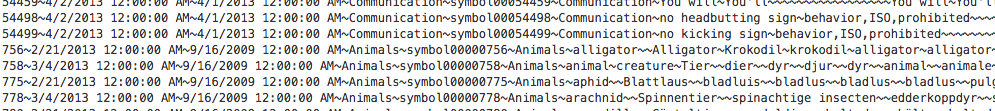
\includegraphics[width=100mm]{datafil} 
\caption{Bilde av dokumentet hvor de ulike symbolene er registrert} 
\label{fig:skrivebord} 
\end{figure} 

//bilder til vært ord var hentet fra internett, ikke bra nok o.
Ettersom det måtte testes og derfor ha mulighet for norsk, så fikk bilder av tobii dynavox, symbolstix. Kommersielt beskyttet. Hadde en annen struktur på bildene. Kun ha laget et script som skrev om til json format. Problem er at tekstdokumentet hele tiden oppdateres. Kunne da ha kjørt scriptet på ny, men fordelene me tekstparser ble for store. Derfor mulighet til begge deler. 

Format til teksten er slik. Se figur blabla. Her har en egenskaper som gjør at en enkelt kan skifte språk. asddas


FOr

//Hvorfor også lage teksttolker
    
    //Var nødvendig for å hente mer filer fra symbolstix filen
    // 
    //kunne ha gjort om filen 


\subsection{Modellene}

Modellene i MVVM mønsteret enkapsulere forretningslogikk og data.Der forretningslogikk er de

The model in the MVVM pattern encapsulates business logic and data. Business logic is defined as any application logic that is concerned with the retrieval and management of application data and for making sure that any business rules that ensure data consistency and validity are imposed. To maximize re-use opportunities, models should not contain any use case–specific or user task–specific behavior or application logic.













//format









Funksjonaliteten som kreves for at en bruker skal kunne skrive setninger kan sammenlignes med et tastatur, men istedenfor bokstaver så er det ord.  



Skrivebordet er representert i koden som KeyboardViewModel mens brukergrensesnittet gjengis KeyboardView. 


//Dataservice
//Innlesning JSONparser / Text-parser
    //Formatet på teksten
    //Oppretter dictionary med symboltabeller
    //Ulempe forward backward
    //Gjør spørring
    




 
 //skriv om all de ulike funksjonene og hvordan de fungererma
 
 
 
 
 
 
 
 
 
 
 
 
 
 
 
 
 
 
 
 
 
 
 
 
\section{SymbolStix} 
 
 
En viktig del av programvaren er å hjelpe barn å bygge et vokabular ved å visualisere ord med bilder. Det vil si at for hvert ord må det finnes et bilde, noe som kan bli svært mange. Tobii Sono Flex har løst denne oppgaven med å bruke et kommersielt tredjeparts bildebibliotek kalt SymbolStix \cite{n2y}, utviklet av n2y. Bildene i biblioteket består av svært enkle tegninger som kun har med det mest nødvendige får å få frem konseptet eller ordet symbolet prøver å representere. Det at Sono Flex og at dette bildebiblioteket var tilgjengelig gjennom Tobii gjorde at den samme bildepakken skulle bli brukt i prototypen. Dette gjorde også medføre at ikke unødvendig med ressurser ble brukt på anskaffe bilder for hvert ord. 
 
 
 
 
\section{Problem} 
 
 
Symbolstix bildene er lagret i Enhanced Metafile Fomat (EMF), som er et 32-bit format som kan inneholde både vektor og bitmap informasjon\cite{AboutEMF}. Problemet med EMF formatet er at det ikke finnes støtte for dette i WPF, med den begrunnelse at det har blitt funnet en kritisk sårbarhet\cite{EMFVulnerability} og at formatet er mer mottakelig for sårbarheter\cite{EMFForum} enn andre bildeformater. I Sono Flex fungerer dette fint, fordi det bygget på Windows Forms(WF),  et rammeverk som har innlagt støtte for EMF. WPF har støtte for å bruke WF elementer,  en funksjon som ble lagt inn for å lette overgangen fra WF til WPF. Som igjen gjorde det mulig å hente bilder med EMF format. Ulempen er at man må trekke inn store deler av WF biblioteket noe som fører til en betraktelig økning i størrelse. For å aktivere støtten, deklarerer en WindowsFormHost i xaml filen og denne vil fungere som en kontainer for alle WF elementer. Innenfor denne kontaineren vil alt fungere som i et WF miljø. Ved å gjøre dette ble alle bildene hentes og vist i prototypen.  
 
 
Testing av applikasjonen viste derimot at det ikke lenger var mulig å trykke på knappene, eller mer korrekt, det var ikke mulig å trykke på  bildet der knappen var. Dette viste seg å være kjent problem, og er kjent som Airspace problemet (kilde) og kommer av at alle WF elementer uansett vil legge seg over alle WPF elementer. Et problem som ikke kunne være med i prototypen. En fix til dette ble laget og planlagt lansert i .NET versjon 4.5, men da versjonen ble lansert, var ikke denne fiksen med. Det finnes ulike omveier rundt på problemet, men få tilfredsstillende.  
 
 
Det ble derfor prøvd å konvertere EMF filene til bitmap for så å vise de i applikasjonen. Fordelen med denne fremgangsmåten var at vi slapp å trekke inn windows forms biblioteket. Ulempen var derimot at hver gang et symbol skulle hentes så måtte dette først konverteres til Bitmap for deretter og rendres. En tidkrevende prosess som gjorde at det tok flere sekunder å laste brukergrensesnittet. Det ble derfor prøvd å konvertere alle filene og deretter lagre dem som jpg. Konverteringen ville da kun gjøres en gang. Deretter ville applikasjonen hente jpg filene direkte, uten noe omvei. Siden wpf har innebygd støtte for formatet. Igjen viste det seg at dette ikke var godt nok ettersom jpg filene hadde blitt for store i overgangen fra vektor til raster grafikk og de manglet gjennomsiktighet. For mens EMF filene lå på under 10kb endte alle de konverterte filene opp på over 100kb. Noe som i selv ikke er så stort, men som gir utslag på lastingen av applikasjonen når det kan være opp mot 200 bilder som skal lastes. 
 
 
Den endelig løsningen ble å laste ned et profesjonelt konverteringsverktøy kalt AVS Image converter. En svært ømfintlig prosess som tok svært lang tid, men som gjorde det mulig å konvertere de orginale EMF filene til png og samtidig holde størrelsen på rundt 10 kb. 
 
 
 
 
 

 
 
\section{Layout} 
 
 
Prototypen har den samme layouten som Tobii Sono Flex, med en menylinje etterfulgt av en symboltabell under. Det er derimot en del variasjoner inne i hver av disse komponentene. 
 
 
\subsection{Menylinjen} 
 
Menylinjen dekker 1/5 del av applikasjonens vindu og består av 4 knapper og listen over ord som brukeren har trykket på. Denne listen vil heretter bli referert til som ordlisten. 
 
 
\subsubsection{Tilbaketasten} 
 
Tasten som befinner seg til høyre for ordlisten er tilbake tasten. Som på et vanlig tastatur vil et trykk på denne knappen medføre at det siste ordet i ordlisten fjernes. 
 
 
\subsubsection{Ordlisten} 
 
Når en bruker trykker på et ordsymbol så vil dette legge seg i ordlisten og når han trykker på "prate" knappen så vil ordene i listen bli gitt gjennom høyttalerne som naturlig tale og deretter fjernes fra listen. Selv om det er plass til uendelig med ord i listen så vil det kun være mulig for brukeren å se maks 4 om gangen. Hvis det allerede er fire symboler i listen når brukeren trykker på et nytt symbol, så vil de tre første bli "fjernet" mens det fjerde og det nye symbolet vil være igjen. Hvis brukeren igjen fjerner de to siste ordene ved å trykke på tilbaketasten,  vil ordene som kommer før igjen bli presentert for brukeren i setningsliseten.  
 
 
\subsubsection{Hjem} 
Ved å trykke på "hjem" knappen vil brukeren alltid bli ført til førstesiden av applikasjonen uavhengig av hvor han befinner seg.  
 
 
\subsubsection{Innstillinger} 
Hvis brukeren første er på "hjem" siden av applikasjonen så vil knappen byttes ut med en "innstillinger" knapp. Ved å trykke på denne vil det åpnes et nytt vindu hvor brukeren vil ha mulighet til å sette og endre på diverse innstillinger. Detaljene rundt denne siden er beskrevet i seksjon. 
 
 
\begin{figure}[ht!] 
\centering 
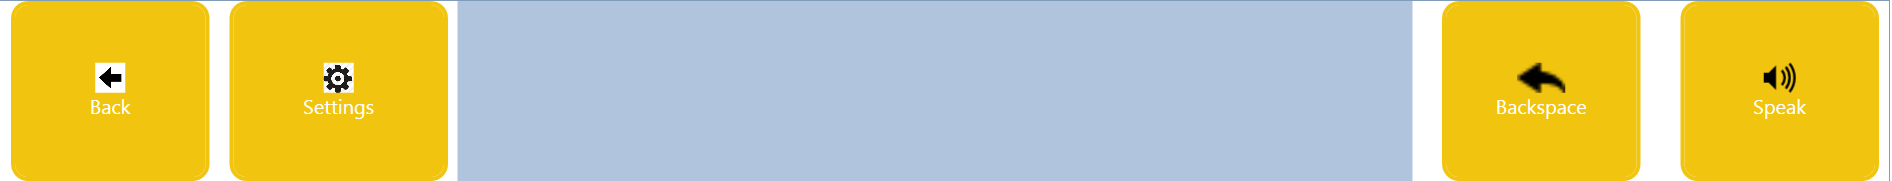
\includegraphics[width=100mm]{MenylinjeP} 
\caption{Skjermdump av menylinjen i prototypen \ref{lst:myLabel}} 
\label{fig:menylinjen} 
\end{figure} 
 
 
 
\section{Symboltabellen} 
 
 
Symboltabellen består av like mange kolonner og rader som den gjør i Sono Flex,  men det er måten den oppfører seg på som er annerledes.   
 
 
 
\section{Oppstart} 
hva skjer når applikasjonen startes. 
Leser fra fil 
Henter bilde2 
 
 
 
 
 
 
\section{Animasjon} 
 
 
Animasjoner i programvare brukes som et virkemiddel for å tiltrekke seg oppmerksomhet, underholde eller demonstrere noe. Det kan enten være en kort animasjon der en knapp tiltrer til en side når man svever over den med musen eller det kan være av den lengre sorten som en flash-video.  Animasjon er i hovedsak alt som beveger seg i applikasjonen. Selv om dynamikken som animasjoner kan fungere som et positivt virkemiddel viser undersøkelser gjort av Nielsen og Loranger \cite{NielsenBok}  at for mye blinkende og bevegende elementer kan slite ut brukeren og gjør det vanskeligere å fokusere på oppgaven. Med animasjonene som er implementer ønsker vi å undersøke dette. Hvilke animasjoner fungerer som et hjelpemiddel og med det gir verdi til applikasjonen og hvilke som er distraherende for brukeren og gir en uønsket effekt. 
 
 
I denne prototypen skjer animasjonene som en respons på at brukeren trykker på et symbol. Hva som skjer avhenger av hvilken type symbol det er. De ulike typene som finnes i symboltabellen ble forklart i seksjon \ref{subsubsec:symboltabell}, og er ordsymbol, kategorisymbol og navigasjonssymbol. 
 
 
 
 
\subsection{Animasjoner: ordsymbol} 
 
 
Når en bruker trykker på et ordsymbol, vil symbolet legge seg i setningslisten og er da klar for gjøres om til tydelig tale. Når brukeren har fullført setningen i Sono Flex blir brukeren presentert for endringen ved at symbolet vises i setningsfeltet. Med prototypen ønsker vi  å gi en mer visuell representasjon av denne endringen til brukeren. Ved å la brukeren kunne velge mellom to animasjoner som oppstår når han trykker på ønsket ordsymbol. De to animasjonene fungerer som følgende: 
 
 
 
 
I) Brukeren trykker på et ordsymbol. 
   Ordsymbolet krympes til 5 prosent av størrelsen. 
   I setningslisten vil en kopi av det krympede ordsymbolet dukke opp. 
   Kopien forstørres så til den opprinnelige størrelsen. 
   Ordsymbolet som opprinnelige ble trykket blir forstørret til opprinnelig størrelse. 
 
 
    
II) Brukeren trykker på et ordsymbol. 
    Ordsymbolet beveger seg ut av sin posisjon og glir mot den posisjonen den vil ha i setningslisten. 
    Når den har truffet posisjonen i setninglisten, stopper den opp og blir værende i ro. 
 
 
    Med disse animasjonen vil en først og fremst gi brukeren beskjed om at et valg har blitt gjort, men de ønsker også gjøre bruk av programvaren mer spennende.  I Sono Flex  vil ingen av knappene ha noe visuelt som gjør at brukeren kan skille hva som skjer, utenom at symboltabellen bytter ut de eksisterende symbolene. I dette tilfelle vil en se at symbolet går fra å være en statisk symbol til å bli flyttet til setningslisten og bli en del av ønsket setning.  
 
 
 
 
 
 
\subsection{Animasjon: Kategorisymbol} 
 
 
Når en bruker trykker på et kategorisymbol vil symbolene i symboltabellen byttes ut med symbolene som hører til i den gjeldene kategorien. Hvis en trykker på kategorien "dyr" så vil tabellen fylles med ordsymbol som "Hund", "katt", "tiger" o.s.v. Her ønsker animasjonen å hjelpe til med å fortelle at man ikke trykker på ordet dyr, men kategorien dyr og at brukeren får en forståelse for forskjellen mellom dem. Animasjonen startet ved at symbolet som brukeren trykket på forstørres helt til den dekker hele symboltabellen. Det vil si at ingen av de andre symbolene vises, kun kategorisymbolet. Symbolet vil så igjen forminskes, men symbolene i tabellen vil være erstattet av symbolene som tilhører kategorien.  
 
 
 
 
\subsection{Animasjon: Navigasjonssymbol} 
 
 
Den siste typen symbol er navigasjon og ved interaksjon vil den navigere mellom sider når det ikke er plass til alle symbolene på en side. Det vil si at symbolet skal kunne navigere fremover, fra side 1 til 2 og 2 til 3 og bakover igjen. Når brukeren trykker fremover starter animasjonen ved at alle symbolene som er på gjeldene side og neste side begynner å bevege seg mot venstre. Slik at symbolene på gjeldene side kontinuerlig blir byttet ut med de på neste. Symbolene på siden sklir ut, mens symbolene på neste sklir inn og overtar plassene. Når brukeren nå trykker på bakover-symbolet vil det samme skje bare at symbolene sklir mot høyre. 
 
 
\section{Lydeffekter} 
 
 
Som en del av rapporten ønsket vi å undersøke hvilken påvirkning lydeffekter hadde på brukeren. Hovedsakelig var målet å finne ut to ting. I hvilken grad hjelper effektene brukeren i å navigere rundt i applikasjonen og om det vil påvirke brukerens helhets uttrykk av applikasjonen.  
 
 
\subsection{Lydeffekter i prototypen} 
 
 
I prototypen er det lagt til flere lydeffekter, utelukkende i form av små lydklipp på maks 1 sekund. Effektene vil kun bli avspilt som en respons til noe brukeren foretar seg eller som å informere om en hendelse. Denne begrensning finnes for å ikke skape forvirring hos brukeren. Hvis lyd også hadde blitt avspilt tilfeldig så ville meningen med effektene forsvinne. Fordi brukeren blir lurt til å tro at programvaren har registrert en interaksjon, selv om han ikke har foretatt seg noe. Det er derfor viktig at det er lett for brukeren å skille mellom effektene som representerer en interaksjon og informasjon. De ulike interaksjonslydeffektene er også forskjellige, og hvilken som blir spilt er avhengig av,  som med animasjon,  hvilken type komponent brukeren samhandler med. Eksempelvis vil lyden som blir avspilt når brukeren trykker å tilbaketasten representere noe som forsvinner.  
 
 
 
 
\begin{itemize} 
\item Symbolord - Enkel klikkelyd 
\item Kategoriord - usikker 
\item navigasjonsord - svisj 
\item Innstillinger - Verktøyskasse 
\item tilbaketasten/slett - forvsinner 
\item hjem - usikker 
\item prat 
\end{itemize} 
 
 
 
 
 
 
 
 
 
 
Dette vil forhåpentligvis gjøre at brukeren mer effektivt kan bekrefte valget og fortsette med oppgaven. Som  
 
 
 
 
 
 
Hvilken brukeren blir presentert for er avhengig av hvilket komponent han interagerer med.  Grunnen er at hvis effektene hadde blit avspilt uten at brukeren foretar seg noe, så kan 
 
 
 
 
Hvilken lyd som blir avspilt er avhengig av hvilket valg brukeren har foretatt seg, og responsen til brukeren vil  
 
 
Eksmepelvis hvis brukeren foretar seg et ulovlig valg vil han bli presentert for en lyd som har gir negative assosiasjoner.  D 
 
 
Lyden som vil bli gitt til brukeren vil komme i form av små lydklipp som maks vil vare i et sekund,  ettersom det skal være nok for at brukeren kan registrere det.  
 
 
 Tilbakemelding i form av lyd gir brukeren en bekreftelse på at han valget han nettopp har foretatt har blitt registrert og  
 

 
Ta for eksempel brødristeren. Når den er ferdig vil brødet hoppe opp, men i tilegg vil den gi fra seg et pling. Altså brukeren vil få tilbakemelding på at han kan hente brødet både visuelt(brødet som hopper opp) og gjennom lyd(plinget). Ved å g 
 
 
Lyd brukes ofte for å fortelle brukeren av produktet noe. For eksempel vil brødristen gi fra seg et pling når den er ferdig samtidig med at skivene hopper opp av maskinen. I dette tilfellet vil  
 
 
 
 
I dag brukes lyd ofte i flere sammenhenger, i alt fra 
 
 
 

 
\section{Sammendrag} 
 
 
 
\chapter{Testing} 
 
 
 
\section{Introduksjon} 
 
 
En viktig del av rapporten var å finne ut hvordan animasjoner og lyd påvirker barns opplevelse av programvaren når de bruker en øyesporingsenhet til interaksjon med maskinen. En fremgangsmåte vil vært å teste på et utvalg studenter og tolke disse resultatene. Problemet er at resultatene ikke nødvendigvis vil være det samme for barn som med voksne. Som tidligere referert, mens barn finner animasjon og lyd interessant og spennende, vil voksne være mindre positive og kan til og med finne dem irriterende. Det ble derfor bestemt at deltakerne i  hvertfall måtte være i nærheten av alderen til målgruppen for at det skulle være noe poeng med testingen. Testen ønsket spesielt å utforske to ting. Den første var å finne ut om målgruppen greide å bruke prototypen. Ville de greie å navigere og utføre de mest nødvendige oppgavene som å skrive en setning, fjerne ord og gjøre det om til tale. Den andre var som tidligere nevnt, å finne ut effekten animasjoner og lyd har når barn skal bruke programvaren.  
 
 

\section{Rekruttering av testere} 
 
 
For å rekruttere deltakere til testen ble først pedagogisk avdeling ved Høgskolen i Bergen kontaktet. De hadde tidligere hatt erfaring med å teste på den ønskede målgruppen. Målet var at disse kunne sette oss i kontakt med nøkkelpersoner og i tillegg gi retningslinjer og tips angående det å bruke barn med funksjonshemninger til undersøkelser. Gjennom dette møte ble vi satt i kontakt med Pedagogisk-psykologisk Tjeneste (PPT). PPT er kommunal tjeneste som skal hjelpe barn, ungdom og voksne som strever i utviklingen, eller som har en vanskelig opplæringssituasjon. Blant annet ved å gi systemrettet støtte, med råd og veiledning til skoler om pedagogisk ledelse av gruppe- og læringsmiljø, og bistand med kompetanse- og organisasjonsutvikling \cite{Udir.5:online}. De hadde god erfaring med målgruppen og hadde et større kontaktnettverk enn høgskolen. Gjennom PPT ble det sendt ut et informasjonsskriv til foresatte av barn som passet inn i målgruppen hvor det ble gjort rede for hvordan undersøkelsen ville bli gjennomført og hvilke og hvor lenge data ville bli lagret. For at testingen skulle gjennomføres, måtte en av barnets foresatte signere og returnere skjemaet. Uheldigvis var det ingen av de foresatte som ønsket at barnet skulle delta i undersøkelsen. 

Vi ble derfor enige om at programvaren uansett måtte testes og at det nærmeste da ville være barn i samme alder som målgruppen, men uten funksjonshemningene. 

Det ble etter en kontaktrunde klart at seks foresatte med barn ved Krohnengen barneskole hadde gitt sin tillatelse til å la barna delta i undersøkelsen. 
 
 
\section{Gjennomføring av test} 
 
 
\subsection{Pilottest} 
 
 
Før testingen ble det utført en pilottest på skolen med 4 medstudenter. Dette ble gjort for at testingen skulle gå best mulig og for å identifisere tekniske feil og eventuelle andre hindringer som kunne oppstå underveis.  
 
 
\subsection{Sted} 
Testen ble utført på Krohengen barneskole inne på biblioteket mellom klokken 13:00 - 
16:00. Bilde \ref{fig:test_lokale} viser et bilde av testrommet. Dette rommet ble valgt fordi det var nært barnas oppholdsrom og fordi det var 
stille. Det var ingen andre barn utenom deltakeren i rommet når testen ble utført. 

 
 
\begin{figure}[ht!] 
\centering 
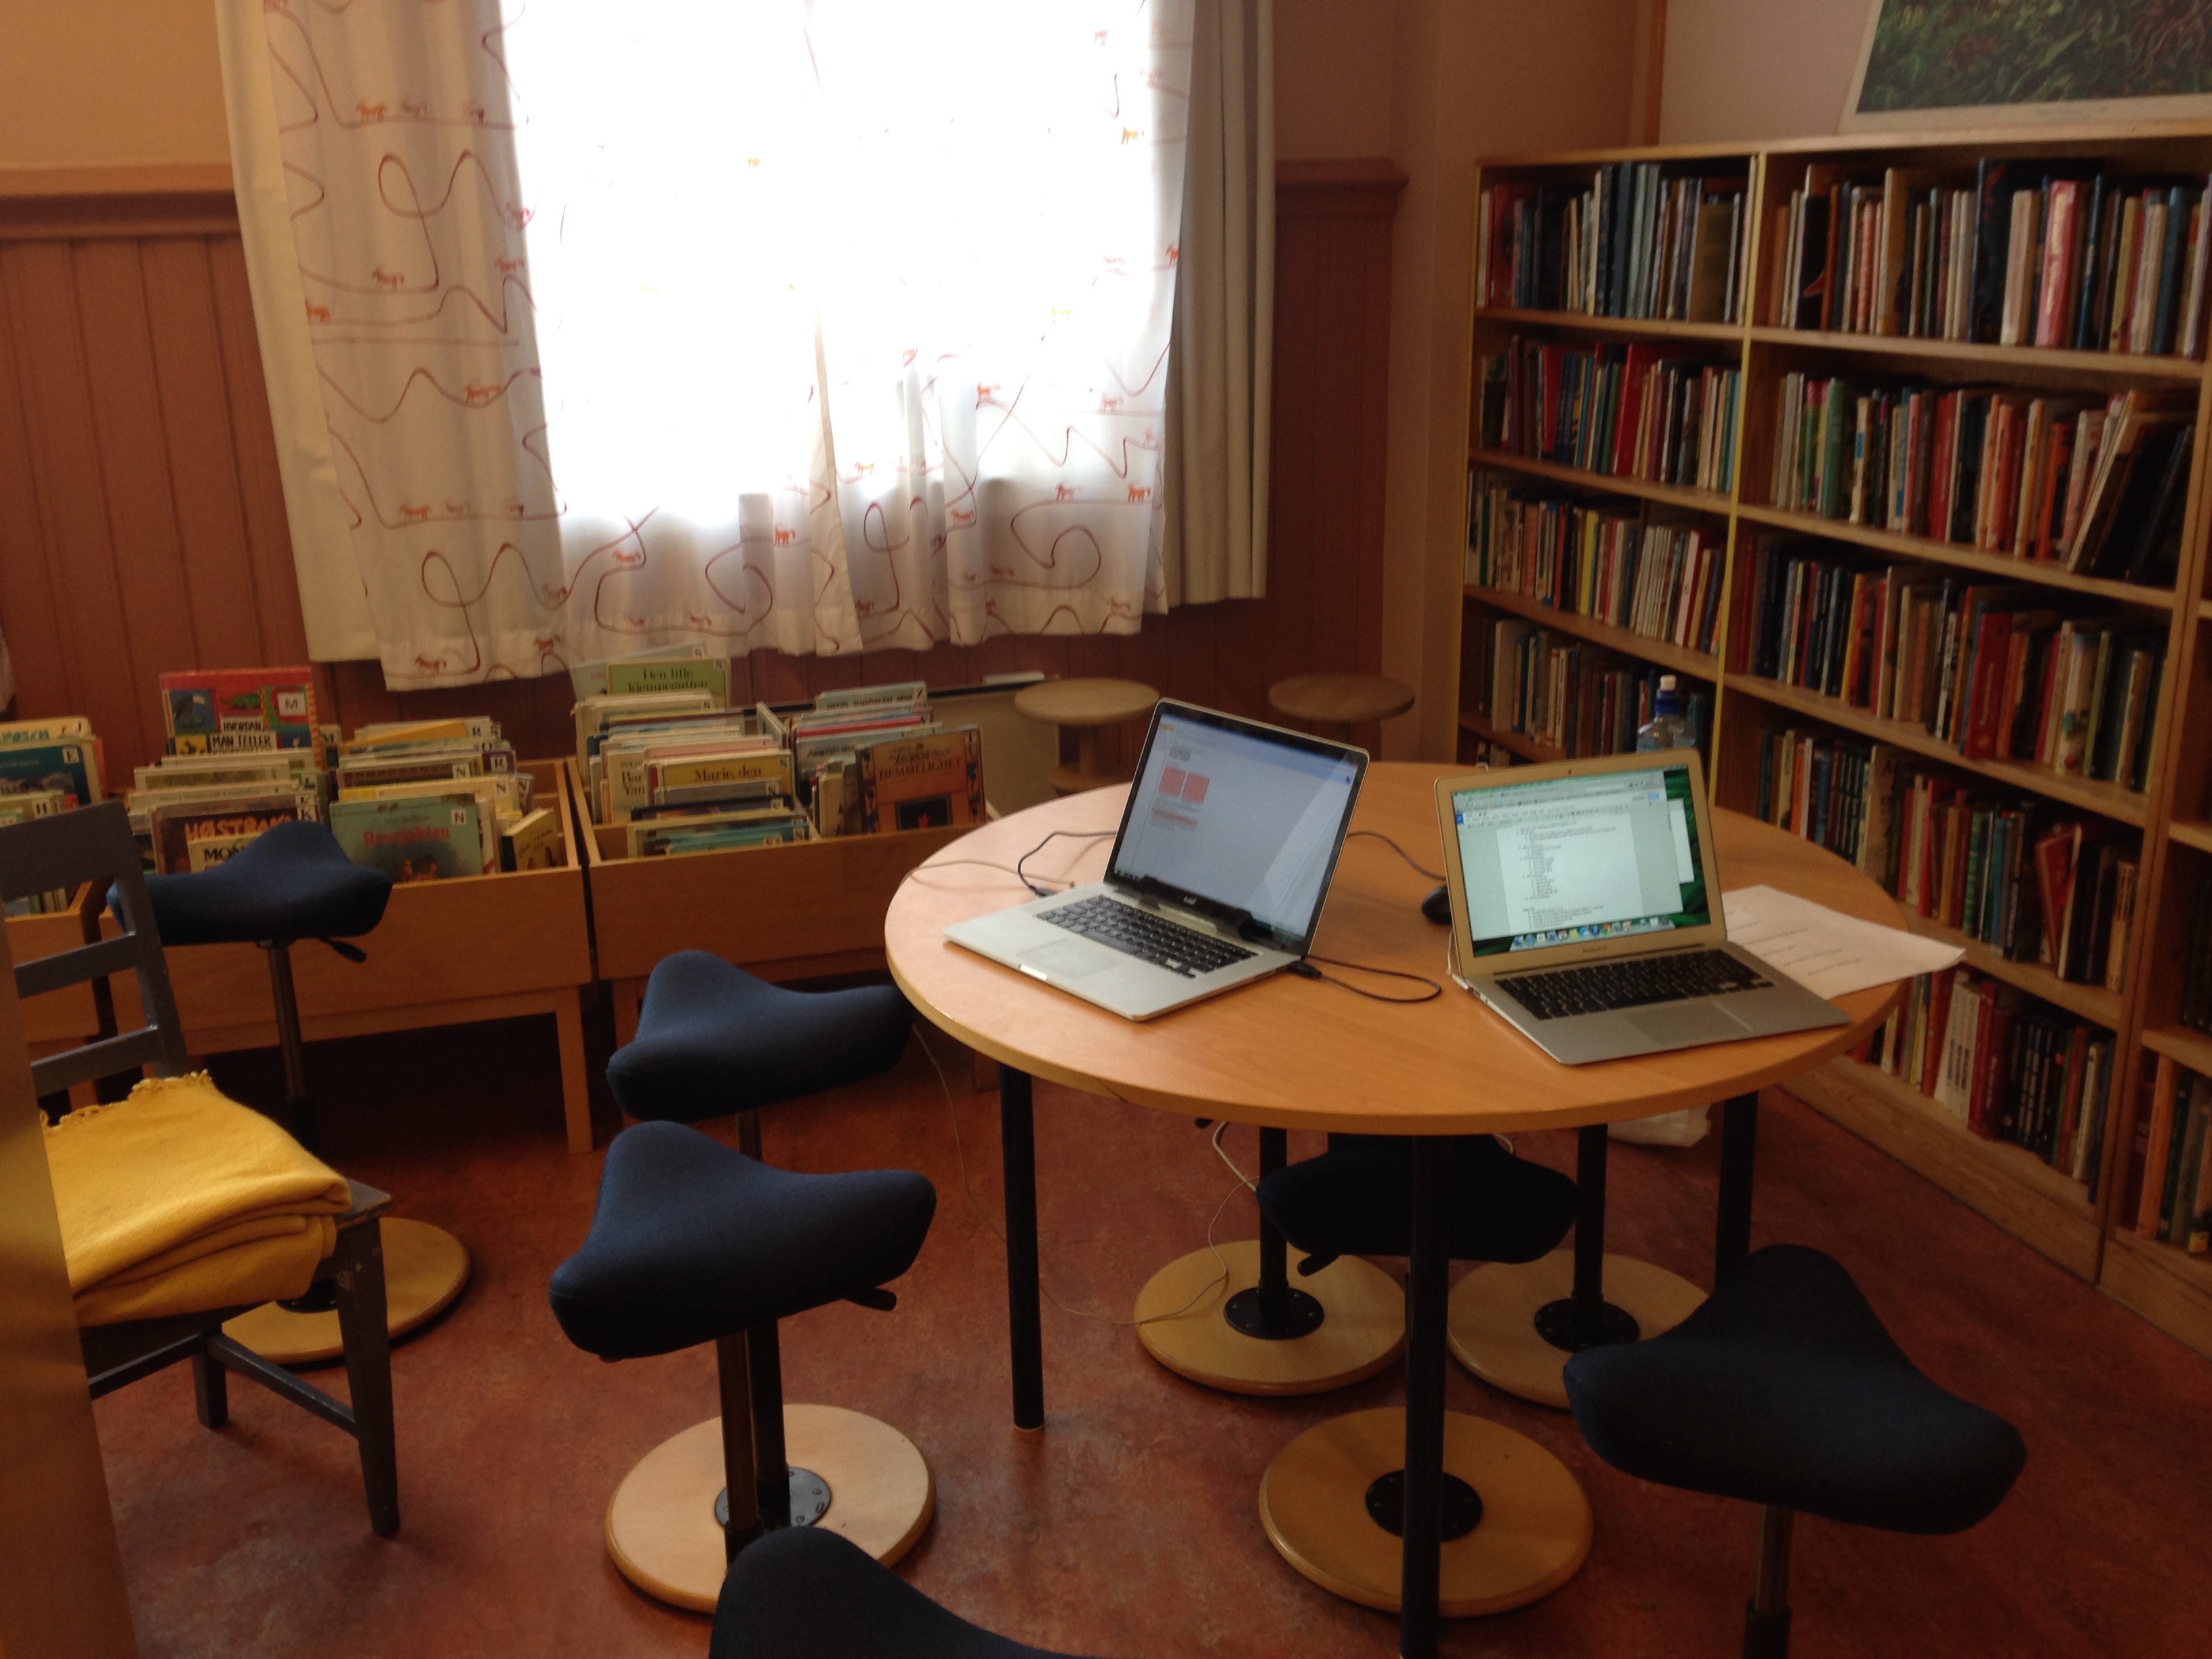
\includegraphics[width=100mm]{Lokale} 
\caption{Bilde av testlokale} 
\label{fig:test_lokale} 
\end{figure} 
 
 
 
 
\subsection{Testgjennomføring} 
Hver test ble gjennomført ved at et og et barn kom inn i biblioteket hvor det først ble foretatt en kort 
samtale for at barnet skulle føle seg komfortabel. For å unngå distraksjoner var kun deltaker og testleder 
tilstedeværende under testingen. Barnet ble så plassert foran datamaskinen og øyesporingsenheten satt slik at den siktet på deltakerens ansikt. For at øyesporingsenheten skulle bli mest nøyaktig måtte den tilpasses for hver deltaker ved en kalibreringsprosess. Prosessen foregikk ved at brukeren følger en rød prikk som starter i 
venstre hjørne og traverserer over skjermen to ganger før den stopper nede i høyre hjørne. Dette 
tar cirka 30 sekund. Etter hver test ble det gitt en farge som beskrev hvor godt enheten greide å 
tilpasse seg brukeren. Rødt er dårligst og programvaren vil ha vanskeligheter med å regne ut hvor 
brukeren ser på skjermen. Gul vil si at kalibreringen gikk greit og at brukeren skal kunne bruke 
enheten på en god måte. Grønn er den mest nøyaktige kalibreringsgraden og enheten vil presist 
fange opp hvor brukeren skuer. Hvis en bruker fikk kalibreringsgrad rød, ble prosessen gjentatt en 
gang. Hvis det igjen viste seg å bli rød ble brukeren bedt om å bruke mus. Kalibreringsgraden ble 
notert for alle brukerne. Deretter ble programvaren startet, og brukeren fikk lov å prøve programvaren før selve testen startet. 
 
 
Testen startet med at brukeren ble  gitt 5 oppgaver som skulle gjennomføres. En bruker ble kun presentert for en ny oppgave når den forrige var fullført. Hver oppgave hadde en makstid på 5 minutter. Det vil si at hvis deltakeren brukte mer enn dette, ville oppgaven bli registrert som feil og avsluttet. Brukeren ville så bli tildelt neste oppgave. Denne makstiden ble valgt utfra pilottestingen. Der brukte deltakerne ca. 30 sekund per oppgave, og med tanke på at disse var i 20 årene ble det også lagt til en god sikkerhetsmargin. Under testingen ble det forsøkt å gi minst mulig spørsmål og ledetråder for å ikke forstyrre eller hjelpe brukeren, ettersom dette ville ha påvirket resultatet. Når brukeren hadde gjennomført alle oppgavene ble han stilt 5 spørsmål. Til slutt ble deltakeren takket for deltakelsen og tildelt et trekk til sykkelsete som kompensasjon. 
 
 
\section{Datainnsamling} 
 
 
For å samle inn data ble det brukt flere ulike metoder.  
 
 
\subsection{Loggfører} 

En viktig del av undersøkelsen var å se hvor lang tid og hvor mange trykk deltakeren brukte på å utføre de forskjellige oppgavene som han ble tildelt. For å gjennomføre dette ble det brukt en logger som lagret data for hver test på separate tekstfiler. Grunnen til at en logger ble brukt er fordi data lagres i et standardformat som gjør at en enkelt kan kjøre spørringer og dermed hente ut målbar data. Data lagres også med en presisjon på tid som en menneskelig observatør ikke har mulighet til og er ikke like mottakelig for feil. Den har også den fordelen at den ligger i bakgrunnen uten brukeren merker noe til den samtidig som den ikke har noen merkbar innflytelse på programvarens ytelse. 
 
 
Så for hver test ble det logget starttidspunktet, om animasjoner er på eller av, alderen til barnet og om den nødvendige kalibreringen er blitt fullført. Deretter var det kun data fra interaksjoner brukeren gjorde med programvaren som ble lagret. Ettersom brukeren kun har mulighet til å trykke på brikker kan det forenkles til at hver gang deltakeren trykket på en brikke ble data logget. Så for vært trykk på en brikke ble det lagret hva som sto på brikken, hvilken type brikken var av og tidspunktet. 
 
 
 
\subsection{Skjermopptak} 
 
Loggeren fanger kun opp interaksjoner deltakeren gjør med programvaren, noe som utelater det som skjer imellom hver interaksjon. For å kompensere for dette ble det bestemt å ta i bruk en skjermopptaker som kunne fange opp hendelser mellom trykk. Noe som kunne være interessant for å se hvor brukeren "nesten" trykket og hvordan han beveget blikket, og generelt andre unntak som måtte oppstå. En stor ulempe med skjermopptak er at en observatør fysisk må se igjennom opptaket for å kunne hente ut informasjon. Noe som kan bli ressurskrevende.
 
Skjermopptakeren ble som med loggeren startet på nytt for hver test og lagret som separate mp4 filer.  
 
 
\subsection{Observasjon} 
 
For å senke terskelen for at foresatte skulle tillate barna å delta i testen ble det valgt å ikke filme barna under testing. Dette gjorde derimot at en ikke fikk med seg reaksjoner eller spørsmål som ble stilt underveis. Så for å kunne fange opp dette ble det brukt en observatør til å notere ned eventuelle hendelser og spørsmål som deltakeren måtte gjøre seg underveis. Ulempen med dette er at man ikke har samme mulighet som med film til å undersøke det i ettertid. Hvis man går glipp av noe er det ikke mulig å spole tilbake for å se det igjen. Det kan også virke forstyrrende på en deltaker at en person noterer det han foretar seg. 

 
\subsection{Intervju} 

Etter at deltakeren har gjennomført oppgavene vil det bli gjort et kort semi-strukturert intervju. Som vil si at spørsmålene er forhåndsdefinerte som i en undersøkelse, men med mulighet for å komme med oppfølgingsspørsmål for å få klarhet i svarene. Intervjuet ble gjort for å undersøke ting som det ikke var mulighet til å fange opp med automatiske verktøy. Blant annet hvordan brukeren opplevde programvaren og hva han syntes om den. 
 
\section{Oppgaver} 

Som en del av testen ble deltakerne gitt oppgaver som går ut på enten å finne frem enkle ord eller kombinere flere ord til å bygge setninger. For at å kunne gi det beste sammenligningsgrunnlaget ble alle deltakerne tildelt de samme oppgavene. 
 
 
Den første oppgaven var å finne ordet "hvordan". Denne brikken ligger på første siden og skal være enkel å finne. Meningen med dette er at deltakeren skal forstå hvordan oppgavene er oppbygd og samtidig få litt selvtillit til de neste oppgavene. 
 
 
Den andre oppgaven var litt verre, den gikk ut på at man skal finne brikken hvor det står "banan". For å finne denne må man trykke inn på kategorien "Mat og Drikke" for så å finne brikken med "banan", som i dette tilfelle vil være på den første siden inne på kategorien. Vanskelighetsgraden vil øke en del fra første oppgaven, men antagelsen var at det skal være enkelt å forstå at en må trykke på kategoriknappen "mat og drikke" for å finne ordet "banan". I hvertfall i motsetning til mer abstrakte kategorier som "verb" og "pronomen". 
 
 
Tredje oppgaven var å finne brikken hvor det står "Elg". På samme måte som med "banan" må man også her først finne den passende kategorien. Antagelsen var også her at det skal være en ganske grei oppgave å finne for barna, med tanke på at den ligger under kategorien "dyr". Forskjellen her i forhold til forrige oppgave er at man ikke vil finne brikken på første siden etter at man har trykket på kategorien "dry", man må navigere seg over til neste side. Dette er om barna forstår konseptet med sidenavigering.
 
 
I den fjerde oppgaven ønsket vi at deltakeren skulle skrive "Jeg vil ha banan", og er med det den første oppgaven hvor deltakeren måtte kombinere ord for å bygge en setning. Det ble derfor valgt en rimelig enkel setning der de to første brikkene "jeg" og "vil ha" er lokalisert på den første siden og det siste ordet har deltakeren funnet en gang før. Dette er gjort for at vanskelighetsgraden ikke skal øke for fort når brukeren skal gå fra å finne et ord til flere.
 
 
Den femte oppgaven gikk ut på at deltakeren skulle skrive setningen "Jeg liker katt". Igjen vil de to første ordene være på første siden. Mens det det ordet "katt" vil finnes under kategorien "Dyr", som barnet tidligere har vært innom i tredje oppgaven når han skulle finne "Elg". 
 
 
\section{Resultat} 
 
 
\subsection{Observasjon} 
 
 
Hver test startet ved at SFO-lederen hentet neste deltaker fra oppholdsrommet og tok dem med til biblioteket hvor undersøkelsen fant sted. De ble så presentert for testlederen av en SFO ansvarlig for at barnet skulle føle seg trygg. Det ble så stilt et par spørsmål, hovedsakelig for å lette på stemningen. Det ble også undersøkt om noen av barna hadde prøvd øyesporing før, noe som hadde gitt dem en stor fordel. Det var derimot ingen av dem som hadde erfaring med øyesporing. 
 
 
Før selve testen startet, ble testdeltaker satt på en stol foran datamaskinen med programvaren og bedt av testleder om å kalibrere øyesporingsenheten. Kalibreringen gikk som tidligere nevnt utpå å følge en prikk som gikk frem og tilbake over skjermen. Her valgte flere av deltakerne å bevege hodet mer enn øyene, og ble dermed bedt om å prøve å holde hodet stille. Flere reagerte på dette med å stirre intenst på prikken som fløyt over skjermen, noe som gjorde at deltakerne i etterkant fikk litt vondt i hodet. I tre av tilfellene gikk kalibreringen så dårlig at den måtte gjentas. Dette virket negativ inn på barna og lagte lyder med negative assosiasjoner. I et tilfelle ble også den andre runden med kalibrering så dårlig at det ikke ville gitt meningen å bruke øyesporing. Det ble derfor bestemt at deltakeren skulle gjennomføre testen med data mus. Dette ble notert og vil bli tatt hensyn til i evalueringen av data. 
 
Når kalibrering var ferdig, ble programmet startet. Her ble deltakeren først presentert for en introduksjonsskjerm og bedt om å velge sin alder av et utvalg på 3 knapper. Her var det flere som med en gang rakk mot styringsflaten for å trykke på knappen med fingrene, ettersom de ikke var vant til å styre med øyene. Det var derimot det eneste tilfelle hvor testleder måtte gjør deltakerne oppmerksom på at de skulle bruke øyene. 
 
Når brukeren var ferdig med introduksjonen starter det som er selve programvaren og som skal testes. Her ble hver deltaker oppfordret til og prøve å trykke på et par knapper med øyene for å bli kjent med følelsen og hvordan interaksjonen fungerte. Den første oppgaven ble så gitt til deltakerne, finn brikken hvor det står "Hvordan". Det kunne da virke som om flere av deltakerne ble litt stresset. For mens de lette rundt på skjermen etter den korrekte brikken så begynte tiden på hver brikke å gå. Det vil si hjulet som sier hvor lang tid som gjenstår før det blir registrert som et klikk. Dette gjorde at de ble tvunget til raskt å flytte blikket rundt for å unngå trykk på uønskede brikker. Det så ut som om tidtakeren som begynner når en bruker ser på en brikke tok veldig mye oppmerksomhet vekk fra den faktiske oppgaven, som var å lete etter rett brikke. Dette gikk igjen under alle oppgavene og gjaldt for alle deltakerne. Dette er nødvendigvis ikke noe som kun gjelder på barn ettersom vi også ble oppmerksom på denne tendensen under pilottesten på eldre deltakere. Opptil flere ganger gikk tidtakeren helt ut på feil brikker, som gjorde at programvaren registrerte det som et trykk og brikken ble flyttet til setningslisten. En deltaker  der animasjoner var slått på, brukte brukeren tid på fjerne feil trykk ved å trykke på tilbaketasten, mens de andre lot feiltrykk være. Testleder ga aldri noen hint om at deltakerne trengte å gjøre dette.  
 
 
Andre oppgaven var å finne ordet "banan", noe som økte vanskelighetsgraden et hakk ved at barnet først måtte finne den passende kategorien, før han kunne finne rett brikke. Som med den første oppgaven begynte de å lete etter brikken i leseretning. Testleder spurte deltakerne under denne oppgaven om å se på bilde eller lese teksten under for å finne rett brikke. Ingen av deltakerne ble forklart at flere av brikkene var kategorier, noe som gjorde at etter å ha sett over alle brikkene kunne opplyse at de ikke kunne finne brikken hvor det sto "banan". Det ble da gitt et tips fra testleder om at noen brikker kunne gjøre slik at det dukket opp flere og at de måtte finne den. Når den var sagt var det ingen som brukte lang tid på finne fram til den korrekte kategorien og deretter finne banan brikken.  
 
 
Etter å ha skrevet banan ble de bedt om å finne brikken hvor det sto elg. Deltakerne så da ut til automatisk å lete blant kategori brikkene og tiden som ble brukt på å finne rett kategori var kort. Problemet var at brikken hvor det sto elg, ikke befant seg på den første siden, men andre. For å komme til denne må en navigere seg til neste side. Her varierte det svært mellom deltakerne. En så blant over alle brikkene og når han ikke fant den ønskede så var han på vei til å navigere seg tilbake istedenfor til neste side. En annen deltaker hadde derimot mer korrekt fremgangsmåte. For etter raskt å ha konstatert at brikken ikke fantes på den aktuelle siden, så trykket han til neste side og fant brikken.  
 
Med de tre første oppgavene unnagjort skulle deltakerne kombinere det de hadde lært ved å skrive den enkle setningen "jeg vil ha banan". Ingen av barna hadde noe særlig problem med å finne de to første ordene, og det tredje hadde alle allerede funnet en gang, men allikevel var det to som ikke automatisk kom på dette og igjen begynte å se over kategoriene. Alle så ut til å håndtere overgangen fra enkle ord til setninger svært bra. Slik at når de kom på tredje oppgaven som var å skrive "Jeg liker katt" så begynte med de med en gang uten noen videre beskjeder fra testleder å finne frem til de korrekte knappene. Til tross for at de ikke hatt brukt brikken "katt" før, så fant de raskt frem rett kategori. Det som var interessant, var at flere valgte feil brikke til tross for at de var på rett side. Grunnen til dette er at inne på første siden finnes det i tillegg til brikken hvor det står "katt" også en brikke hvor det står "kattunge". Det som skjedde var at samtlige av testdeltakerne valgte sistnevnte. På spørsmål fra testleder om hvorfor de gjorde dette, så var det en så svarte at oppgaven var å finne "katt". Deltakerne ble derfor spurt om de baserte brikketrykkene sine på teksten eller bildet. Hvor samtlige av barna svarte at bildet. Noe som ikke bare forklarte hvorfor de valgte "kattunge", men også hvorfor det virket lettere for deltakerne å finne kategorien "dyr" enn "mat og drikke". For mens "dyr" var representer med ulike dyr, så var "mat og drikke kun representert av drikkevarer. Noe vi ble oppmerksom på i etterkant. 
 
Til tross for at ingen av deltakerne hadde brukt øyesporing før, fikk alle det til, med unntak av deltakeren der kalibrering ikke fungerte. Ingen feil dukket opp, og alle deltakerne greide å gjennomføre oppgavene. Selv om det var relativt få oppgaver greide de dem uten noe særlig behov for å tenke seg om. Utfra observasjonene kan en slå fast at for en førstegangsbruker så kan tidtakeren som vises gå litt for raskt og en bør muligens se på alternative måter å vise denne. Ettersom det skjedde flere feiltrykk og deltakerne ble stresset og ikke visste hvor de skulle hvile blikket mens de lette etter ønsket ord. Det kan også slå fast at de i hovedsak bruker bildet til å finne rett brikke noe som gjør at bildet bør vise klart hva det representerer og unngå tvetydighet.  
 

\subsection{Intervju} 
 
Med det semi-strukturerte intervjuet ønsket vi å finne ut hvordan barna opplevde å bruke prototypen. Problemet var at uansett hvordan spørsmålet ble formulert var deltakerne utelukkende positive. Eksempelvis så ga alle karakteren 10 på en skala fra 1 til 10, og på oppfølgende spørsmål om det var ingenting som burde vært annerledes, så var svaret nei. Dette gjorde at flere av spørsmålene som ble stilt ble forkastet.  
 
Et spørsmål som var av interesse var når testlederen spurte barna om de visste hva som skjedde ved å trykke på de ulike knappene. Det vil si om de forsto om det var et ord eller kategori. To av dem svarte klart at ved å trykke på en kategori knapp så ville de knappene bli byttet ut med nye knapper. Mens ved å trykke på et symbol som representerte et ord, så ville det gå opp i setningslisten. De andre greide derimot ikke å svare på dette spørsmål og greide ikke å skille mellom de ulike knappene. 
 

\subsection{Tid} 
 
 
En ting som vi ønsket å finne ut var hvorvidt animasjoner gjorde at deltakerne brukte lengre tid per oppgave eller ikke. For å finne ut dette ble tiden hver deltaker brukte per oppgave registrert.  
 
 
\begin{figure}[ht!] 
\centering 
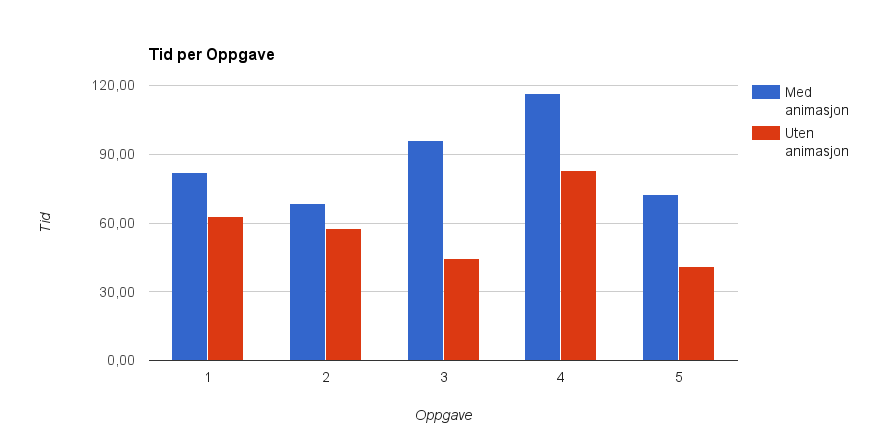
\includegraphics[width=100mm]{TidPerOppgave} 
\caption{Gjennomsnittlig tid per oppgave basert på om animasjoner var på eller ikke.} 
\label{fig:DiagramTidPerOppgave} 
\end{figure} 
 
 
I Diagrammet \ref{fig:DiagramTidPerOppgave} viser den blå søylen den gjennomsnittlige tiden det tok for deltakerne som hadde på animasjoner å gjennomføre oppgaven, mens den røde viser hvor lang tid det tok for de uten. Som man kan se utfra denne så ser man at tendensen er at de som hadde på animasjoner brukte lengre tid en de uten. Noe som kan tyde på at animasjoner gjør at en bruker lengre tid ved å ha animasjonene slått på.  
 
 
 
\section{Tolkning av resultat} 
 

Det er viktig å poengtere at testen kun hadde 6 deltakere og noe som ikke grunnlag for konklusjon og dataene vil i beste fall kun gi indikasjoner.  Med testingen ønsket vi å undersøke hvorvidt målgruppen greide å utføre de mest nødvendige oppgavene i prototypen og hvilken påvirkning animasjoner og lyd hadde på barnet.  
 
Deltakerne hadde ingen erfaring med bruk av øyesporingsenheten eller lignende programvare. Allikevel tok det ikke lang tid før de tilpasset seg og trykket på de forskjellige symbolene. De hadde ingen spørsmål rundt hva som regnet som et klikk eller hva de ulike menyknappene betydde. Deltakerne greide også å gjennomføre alle oppgavene de ble tildelt. En liten oppdagelse ble derimot gjort, alle deltakerne hadde problemer med at timeren, som viser på symbolet hvor lenge det er igjen til det blir regnet som et trykk, gikk altfor fort. Dette var også en erfaring som ble gjort under testingen på medstudenter.  Det var derimot ikke nok til å hindre deltakerne i å operere programvaren og gjennomføre alle oppgavene.

Spørsmålet blir da hvorvidt man kan si om barn i målgruppen kunne utført de mest nødvendige operasjonene på prototypen, med tanke på at deltakerne som ble testet var barn, men uten noen form for funksjonsnedsettelse. Forskjellen er at målgruppen har en funksjonshemning. 

Selv om vi hadde fått testet på målgruppen hadde dette vært en usikkerhetsfaktor, ettersom det finnes flere funksjonshemninger og flere grader av dem. Slik at det man kan si utfra testingen er barn i 6 års alderen har ingen store problemer med å skrive og finne frem til de korrekte ordene og man kan derfor fastslå at et barn i målgruppen også vil hatt mulighet om ikke like lett kunne uttrykke seg selv gjennom prototypen. 
 
I tillegg vil testen også finne ut hvilken effekt animasjoner og lyd ville ha. For å finne ut dette ble data samlet mens deltakerne utførte 6 oppgaver som ble tildelt. Dataene er presentert i diagram og gir klare indikasjoner på at deltakerne som hadde animasjoner og lyd brukte lengre tid på oppgavene enn de uten. Dette er interessant, men det skal igjen nevnes at i tillegg til at det var kun 6 deltakere var det også kun 6 oppgaver som de gjennomførte. Til tross for at de brukte lengre tid på å gjennomføre oppgavene, var det kun de 2 av 3 som hadde animasjoner på som kunne svare hva som skjedde ved å trykke på en kategori- og ordsymbol. Hvis dette skulle stemme så kan det tyde på at en bruker kanskje burde starte med å ha animasjoner på for så etter en stund skru dette av.  
 
Som en oppsummering så kan en si at med så lite testpersoner så kan man ikke si noe sikkert, men vi kan konkludere med at prototypen fungerer og at et barn i seks år alderen enkelt greier å uttrykke seg via denne. I tillegg er det indikasjoner på at animasjoner gjør at en ny bruker av programvaren bruker lengre tid enn uten animasjoner. Det er også indikasjoner på animasjoner og lyd gir brukeren en bedre forståelse for hva de ulike typene symbol representerer.  
 

 

 
 
 
 
 
 
 
 
 
 
 
 



\section{UTKAST: ikke les}


Som med animasjon kan lyd både virke for og i mot sin hensikt. Horanger og Nielsen fant ut under testing av nettsider at ungdommer og voksne fant kvitre og kime lyder var irriterende, men at de appellerte til barn. 

Sammen med animasjoner kan lyder i programvare være effektive til å gi brukeren tilbakemelding på en handling. Eksempelvis kan lyder brukes til varsle brukeren om at de har gjort et feil valg \cite{}, men som med animasjoner vil for mange lyder og uventede lyder være distraherende og irriterende. Nielsen og Loranger fant 




I prototypen ønsker animasjonen å vise hva som skjer,  ved at symbolet beveger seg fra opprinnelige posisjon til set

I Sono Flex dukker symbolet bare opp i setningslisten.

I symboltabellen er det 3 forskjellige typer. Man har 
ordsymbol, kategorisymbol og navigasjonssymbol. Et ordsymbol representerer selvsagt et ord og vil legge seg i listen sammen med andre ord som vil bli 

For å vise hva som skjer, fremfor at det bare skjer. I den eksisterende løsningen Sono Flex var det ingen for animasjoner. Slik at når brukeren trykte på en knapp, skjedde responsen umiddelbart. Man kan si at animasjonene skal representere det som skjer med dataen. Eksmepelvis hvis brukeren trykker på en knapp 


//tre ulike knapper
    //Trykk på knapp
    //neste side
    //Organisasjon



Det vil derfor være viktig at animasjonene som er implementert gir verdi til applikasjonen fremfor å distrahere.

Det vil derfor være viktig å finne ut om animasjonene gir noe verdi 

Interaksjonsdesigneren Nielsen har gjort flere undersøkelser på hvordan en skal få optimal brukervennlighet på webapplikasjoner. 

Animasjoner i programvare og nettsider blir ofte snakket om i negative ordlag fordi de

for det de ofte blir brukt overdrevet mye og er u

Animasjoner blir ofte sett på som en distraksjon når det blir brukt i applikasjoner for det de fjerner fokuset fra det som er viktig. Som 


For å kunne sjekke hvordan animasjon påvirket et barns evne til å samhandle med applikasjonen, måtte de ble implementert.  

//visualiserer at symbolet går fra griden til output, hjelper barnet
// Vanskeligheten med å skaffe empirisk data


Dataanimasjon, animasjonsfilmteknikk som gjør bruk av elektronisk databehandling for å skape illusjon av bevegelse, har fått en svært sentral plass innenfor reklamefilm og fjernsyn. Her har utviklingen gått fra enkle todimensjonale tegninger til avansert 3-D-animasjon som ikke kan fremstilles på andre måter enn med datamaskin.

Ifølge Store norsk leksikon defineres animasjon som levendegjørelse, besjeling, oppmuntring, tilskyndelse. 


Applikasjonen tilbyr flere animasjoner som brukeren kan velge mellom, enten alene eller flere i kombinasjon. Noen animasjoner kan ikke være operative samtidig ettersom det vil føre til konflikt. 

\subsection{Fade in, fade out}

Gjør rede for og forklar de ulike animasjonen

\section{Navigasjon}
Gjør rede for og forklar de forkjellige navigasjons hjelpemidlene

\section{Personlig tilpasning}
Forklar hvordan applikasjonen legger til rette for brukeren.
    - Temaer, forkjellige farger, lyder, 
    - Bruker kan velge hvilke animasjoner som ønskes og hurtigheten på dem.
    
\section{Lyd}
    Gjør rede for de ulike lydene.

\chapter{Dette er bare utkast og stikkord}

Rapporten vil ikke gi noen videre beskrivelse av C-Sharp, derimot vil WPF bli forklart.


\section{Teknologier}

Øyesporingsenheten beskrevet i kapittel  krever at systemet kjører på operativ systemet Windows og APIet som det leveres enheten leveres med,  fungerer kun i programmeringspråkene C-Sharp og C++. Med dette som utgangspunkt ble resten av teknologivalgene er basert på anbefalinger fra dokumentasjonen og tidligere erfaring. 


\begin{description}
  \item[IDE] Visual Studio
  \item[Rammeverk] .NET
  \begin{description}
     \item[Programmeringspråk] C\#
     \item[Grafikk] Windows Presentation Foundation 
\end{description}
  \item[Versjonskontroll] Git (BitBucket)
\end{description}


Fitzergald key, personliggjør keyboardet med farger. Viktigste er at det er konsistent


For å kunne bruke symboler som en kommunikasjonsform kreves det at brukeren har mulighet til samhandle med dem. For å få til dette brukes det en øyestyringsenhet koblet til en datamaskin som fanger opp brukerens pupill bevegelser. På den måten erstatter øyene den vanlige musepekeren.

\subsubsection{Kalibrering}


Første gang en kobler øyestyringsenheten til maskinen, anbefales det at brukeren gjør en oppmåling og kalibrering for mer presis øyesporing. Oppmålingen innebærer at personen måler størrelsen på skjermen - kalibreringen at det brukeren bes om å følge en prikk som traveserer skjermen. Ettersom dette vil gi øyestyringsenheten et referansepunkt. Prosessen er kun nødvendig første gang for gjeldene bruker. 






Dette gir tilgang på deres application programming interface (API), herved referert til som Tec API. Tec API gjør funksjoner og informasjon fra sporingsenheten tilgjengelig. 


The Tobii Eye Control API provides two alternative access points: a .NET assembly and a C dynamic-link library. Both alternatives
give the developers of eye controlled applications access to the functionality of the Gaze Interaction Server. The .NET API also
contains specialized interaction support for common user interface frameworks such asWindows Presentation Foundation
(WPF) andWindows Forms. The C interface, called MPACI, provides backward compatibility with older Tobii products such as
the MyTobii software.




\subsection{Systemkrav}

\subsection{Nøkkelfunksjoner og konsepter}

\section{}



Første gang en kobler til må en gå igjennom ett oppsett. Dette innebærer måling av den aktuelle skjermen som brukes og en kalibrerings rutine. For å oppnå nøyaktig øyesporing.  

For en førstegangsbruker av enheten anbefales det å gjøre en kalibrering, for optimal opplevelse. Informasjonen


Øyestyringsenheten som er illustrert i figur \ref{fig:tobiiPc}  . Denne




\medskip

\bibliographystyle{chicago}%Used BibTeX style is unsrt
\bibliography{sample}

\end{document}
